\documentclass[11pt]{article}
\usepackage{cite}

\usepackage{hyperref}
%biblio
\usepackage{natbib}
\usepackage{url}
\usepackage{wrapfig}

%Math
\usepackage{amsmath}
\usepackage{amsfonts}
\usepackage{amssymb}
\usepackage{amsthm}
\usepackage{ulem}
\usepackage{stmaryrd} %f\UTF{00FC}r Blitz!

%PageStyle
%\usepackage[ngerman]{babel} % deutsche Silbentrennung1
\usepackage[utf8x]{inputenc} 
\usepackage{fancyhdr, graphicx}
\usepackage{subcaption}
\usepackage[scaled=0.92]{helvet}
\usepackage{enumitem}
\usepackage{parskip}
\usepackage[a4paper,top=2cm]{geometry}
\setlength{\textwidth}{17cm}
\setlength{\oddsidemargin}{-0.5cm}
\usepackage{lastpage} % for getting last page number
\renewcommand{\familydefault}{\sfdefault}
\usepackage{setspace}
\usepackage{acronym}


% Code listenings
\usepackage{color}
\usepackage{xcolor}
\usepackage{listings}
\usepackage[font=it]{caption}
\DeclareCaptionFont{white}{\color{white}}
\DeclareCaptionFormat{listing}{\colorbox{gray}{\parbox{\textwidth}{#1#2#3}}}
\captionsetup[lstlisting]{format=listing,labelfont=white,textfont=white}
\lstset{
 language=Java,
 basicstyle=\footnotesize\ttfamily, % Standardschrift
 numbers=left,               % Ort der Zeilennummern
 numberstyle=\tiny,          % Stil der Zeilennummern
 stepnumber=5,              % Abstand zwischen den Zeilennummern
 numbersep=5pt,              % Abstand der Nummern zum Text
 tabsize=2,                  % Groesse von Tabs
 extendedchars=true,         %
 breaklines=true,            % Zeilen werden Umgebrochen
 frame=b,         
 %commentstyle=\itshape\color{LightLime}, Was isch das? O_o
 %keywordstyle=\bfseries\color{DarkPurple}, und das O_o
 basicstyle=\small,
 stringstyle=\color[RGB]{42,0,255}\ttfamily, % Farbe der String
 keywordstyle=\color[RGB]{127,0,85}\ttfamily, % Farbe der Keywords
 commentstyle=\color[RGB]{63,127,95}\ttfamily, % Farbe des Kommentars
 showspaces=false,           % Leerzeichen anzeigen ?
 showtabs=false,             % Tabs anzeigen ?
 xleftmargin=17pt,
 framexleftmargin=17pt,
 framexrightmargin=5pt,
 framexbottommargin=4pt,
 showstringspaces=false      % Leerzeichen in Strings anzeigen ?        
}

%Config
\fancypagestyle{firststyle}{ %Style of the first page
 \fancyhf{}
 \fancyheadoffset[L]{0.6cm}
 \lhead{
 
\includegraphics[scale=0.8]{./fhnw_ht_e_10mm.jpg}}
 \renewcommand{\headrulewidth}{0pt}
 \lfoot{Institute 4 Data Science,\linebreak www.fhnw.ch }
}

\fancypagestyle{documentstyle}{ %Style of the rest of the document
 \fancyhf{}
 \fancyheadoffset[L]{0.6cm}
\lhead{
 
\includegraphics[scale=0.8]{./fhnw_ht_e_10mm.jpg}}
 \renewcommand{\headrulewidth}{0pt}
 \lfoot{P7 Radio Interferometry with Compressed Sensing}
 \rfoot{\thepage\ / \pageref{LastPage} }
}

\fancypagestyle{tableofcontent}{ %Style of the rest of the document
 \fancyhf{}
 \fancyheadoffset[L]{0.6cm}
\lhead{
 
\includegraphics[scale=0.8]{./fhnw_ht_e_10mm.jpg}}
 \renewcommand{\headrulewidth}{0pt}
 \cfoot{\thepage}
}

\fancypagestyle{abstract}{ %Style of the first page
 \fancyhf{}
 \fancyheadoffset[L]{0.6cm}
 \lhead{
 
\includegraphics[scale=0.8]{./fhnw_ht_e_10mm.jpg}}
 \renewcommand{\headrulewidth}{0pt}
 \cfoot{}
}


%Metadata
\numberwithin{equation}{section}


\begin{document}
\title{Radio Interferometry with Compressed Sensing}
\author{Jonas Schwammberger}
\date{Today}
\maketitle

\newpage
\pagestyle{abstract}
\section*{Abstract}
Reconstruction from under-sampled measurements, Theory of Compressed Sensing tells us how it is done. Theory was applied on measurements from radio interferometers which naturally produce under-sampled measurements. 

%TOC
\newpage
\pagestyle{tableofcontent}
\pagenumbering{Roman}
\tableofcontents  	
\newpage

\pagestyle{documentstyle}
\setcounter{page}{1}
\pagenumbering{arabic}

\section{Interferometry and the Inverse Problem}\label{intro}
Astronomy requires its instruments to have a high angular resolutions. This is an issue for radio wavelengths: The longer the wavelength, the bigger the diameter of a single dish antenna. Single dish antenna's are expensive to build and harder to steer accurately. Interferometers, where multiple smaller antennas act as a single large instrument, can achieve high angular resolutions while being cheaper to build. In the past, interferometers like VLA, AlMA and LOFAR have made numerous discoveries.

Interferometers do not observe the sky directly. Each antenna pair measure Fourier Components (Visibilities) of the sky brightness. The observed image has to be reconstructed from the measured Visibilites. Since the interferometer can only observe a limited number of Visibilities, the reconstruction is an ill-posed inverse problem. For small Field of View imaging, the CLEAN class of Algorithms\cite{hogbom1974aperture}\cite{schwab1984relaxing}\cite{rich2008multi}\cite{rau2011multi} have been developed and is the de-facto standard in Radio Astronomy. It is not guaranteed to reconstruct the true image in theory. In practice it has produced remarkable results with expert tuning. New generation Interferometers like ASKAP, Pathfinder and SKA are built with wide Field of View imaging in mind. The CLEAN Algorithms have been extended for Wide Field of Views, but require even more tuning by experts. 

The Theory of Compressed Sensing\cite{many} has seen success in solving ill-posed inverse problems. It is flexible in its application and has produced remarkable results image de-noising\cite{many}, in-painting\cite{many} and super-resolution\cite{many}. Applying Compressed Sensing to wide Field of View imaging is an active field of research. In the last decade numerous approaches have been developed showing the potential of Compressed Sensing: Accurately modelling the effects of wide Field of View imaging, while reducing the tunable parameters and possibly super-resolved images\cite{many}. Current research focuses on how the effects of wide Field of View can be accurately modelled while still being computationally efficient.

In this project, a proof of concept Compressed Sensing approach was developed and implemented in the Common Astronomy Software Application(CASA). The approach is focused on small Field of View imaging and the reduction of expert intervention.

\subsection{Inverse Problem for small Field of View Imaging}
Each antenna pair measures a complex Visibility of the sky brightness. The distance between the antennas, the baseline, dictates the sample point in the Fourier Space (called UV-Space). Longer baselines sample higher frequency components, while shorter baselines sample lower frequency components. 

For small Field of View imaging, the measured Visibilities equal two dimensional Fourier components. The observed image can be calculated by the two dimensional Inverse Fourier Transform. However the interferometer cannot sample the whole UV-Space. The image calculated by the Inverse Fourier Transform is 'dirty', it contains artefacts introduced by undersampling. 

\begin{figure}[h!]
	\centering
	\begin{subfigure}[b]{0.28\linewidth}
		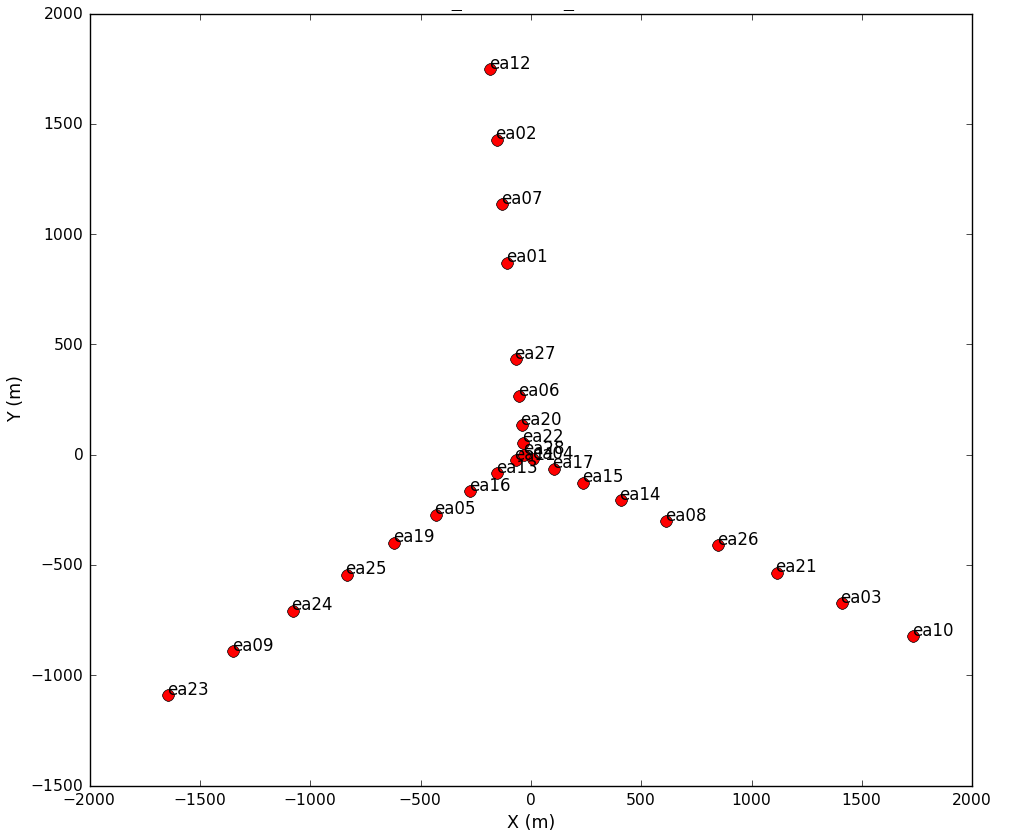
\includegraphics[width=\linewidth, trim={18px 19px 18px 18px}, clip]{./chapters/01.intro/img/antennas.png}
		\caption{Antenna Configuration}
	\end{subfigure}
	\begin{subfigure}[b]{0.28\linewidth}
		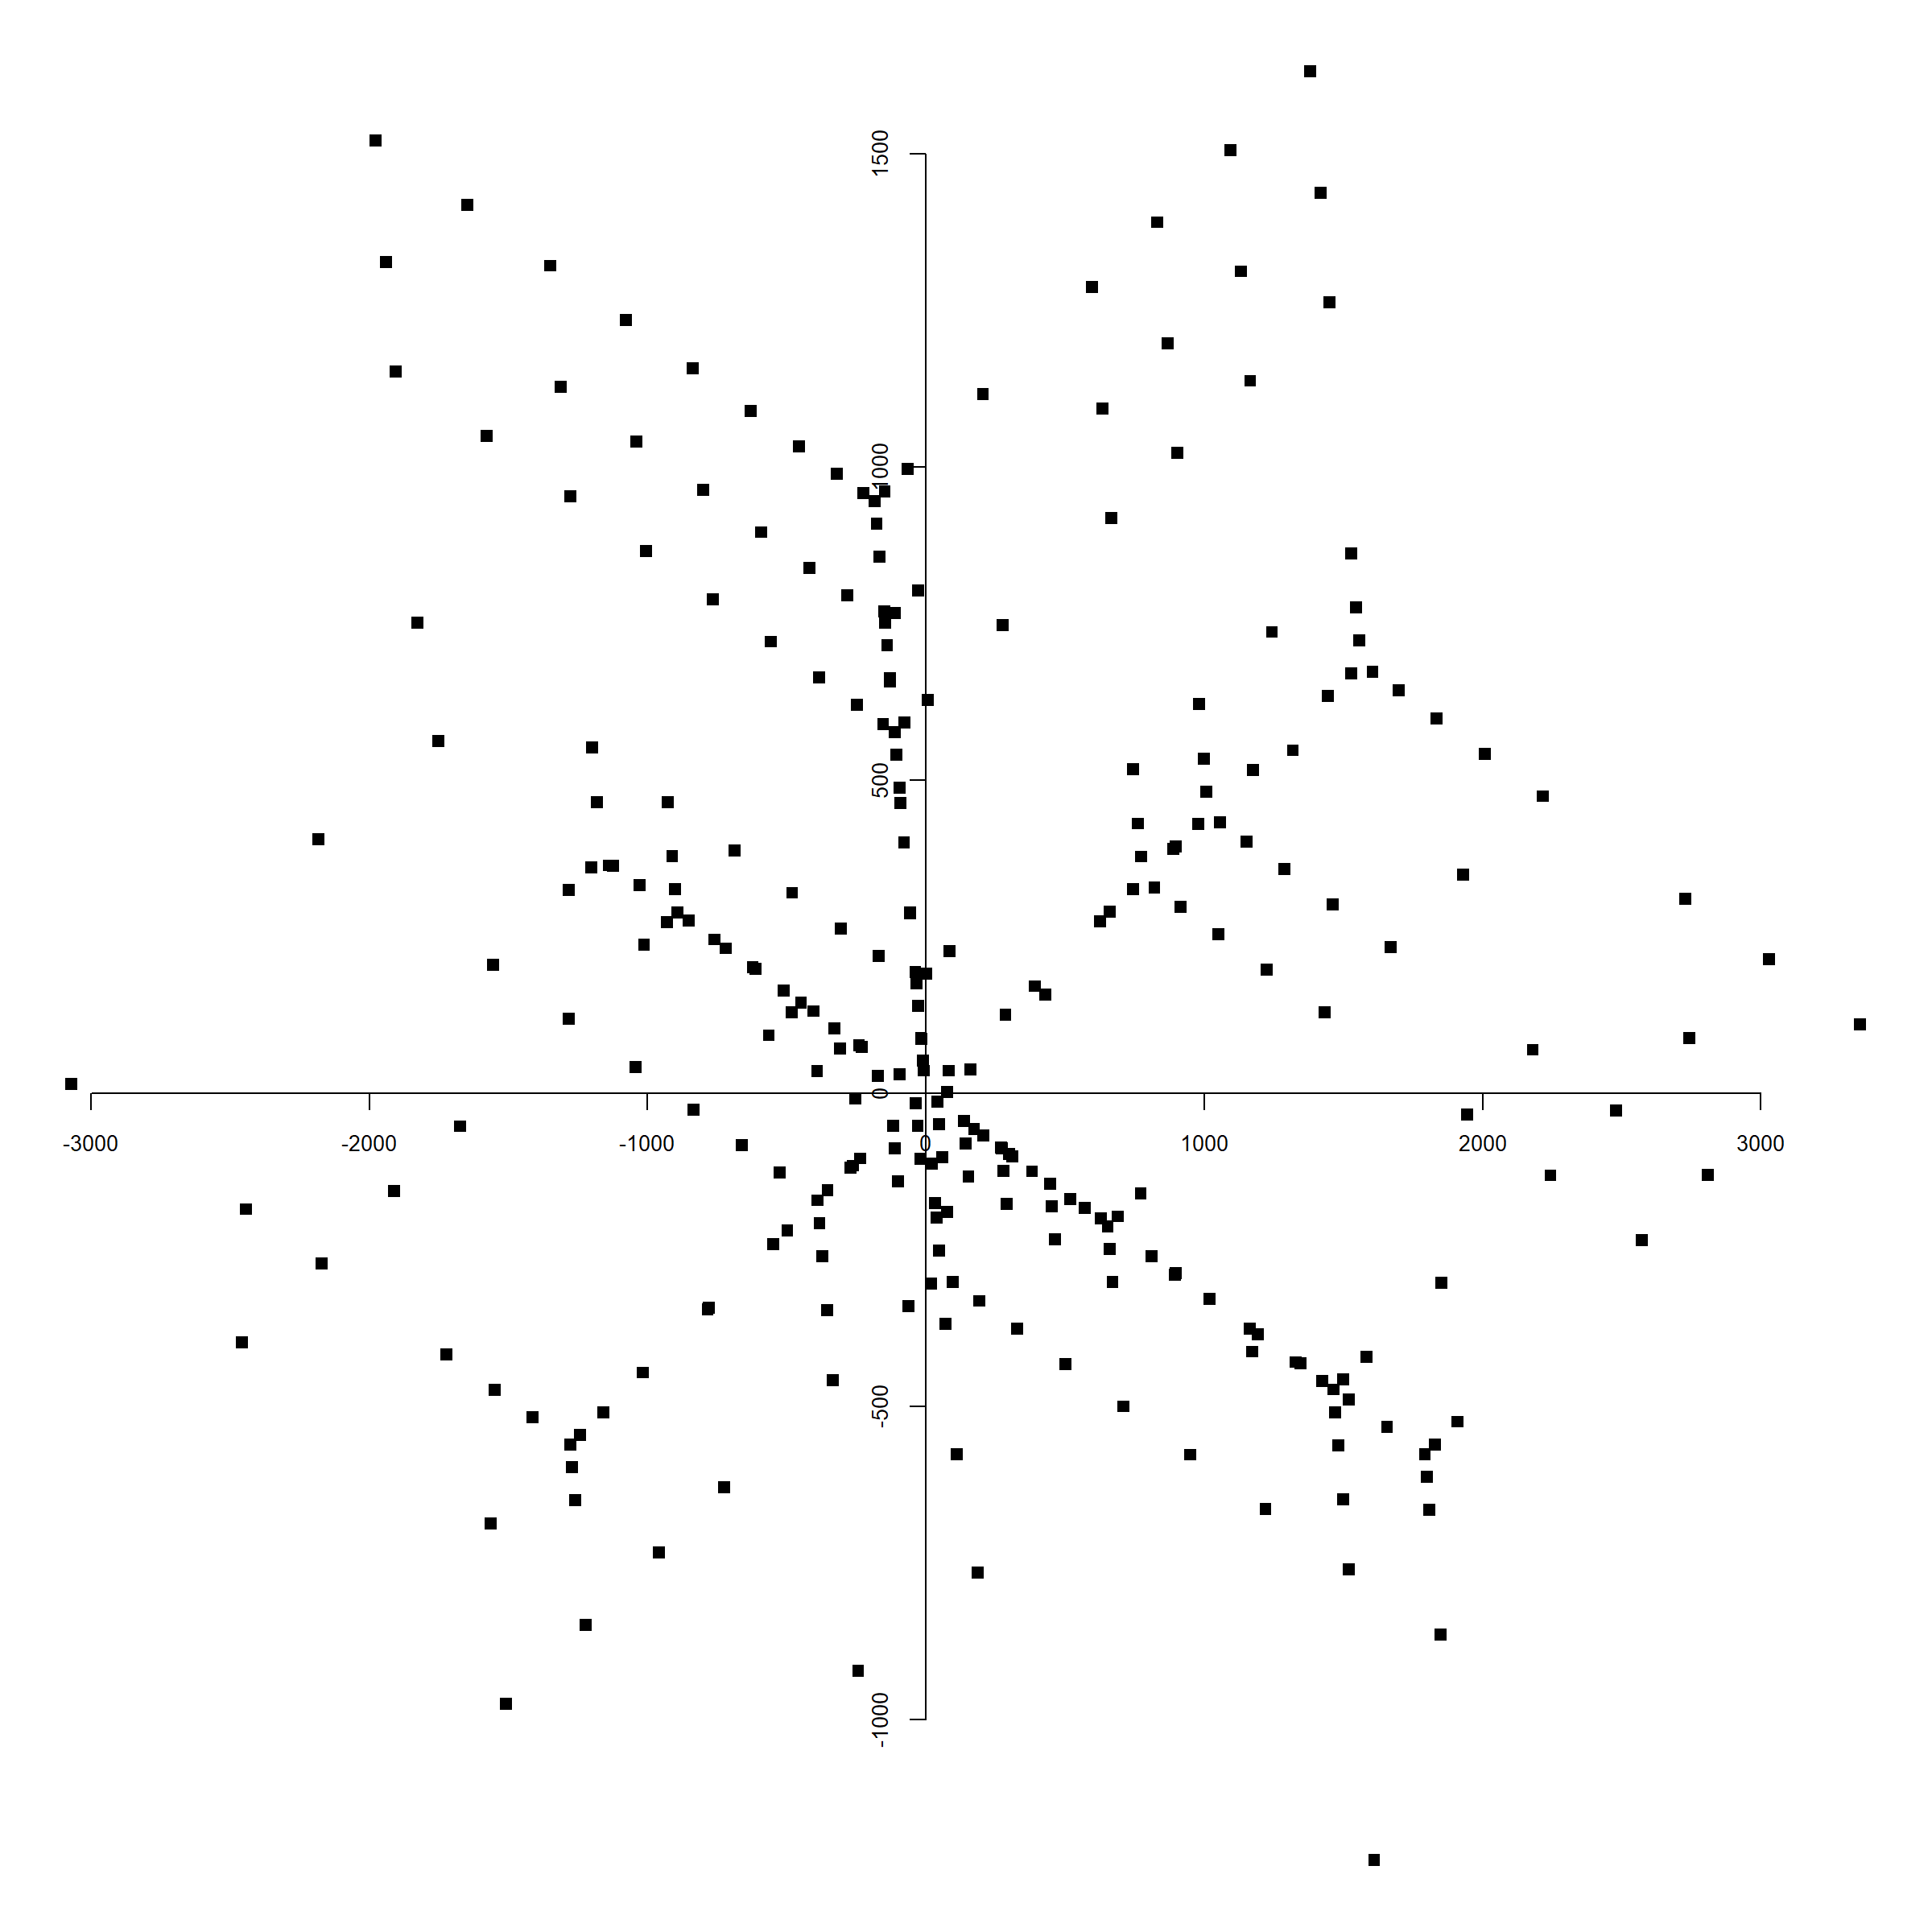
\includegraphics[width=\linewidth, trim={18px 19px 18px 18px}, clip]{./chapters/01.intro/img/uv.png}
		\caption{UV-Space}
	\end{subfigure}
	\begin{subfigure}[b]{0.28\linewidth}
		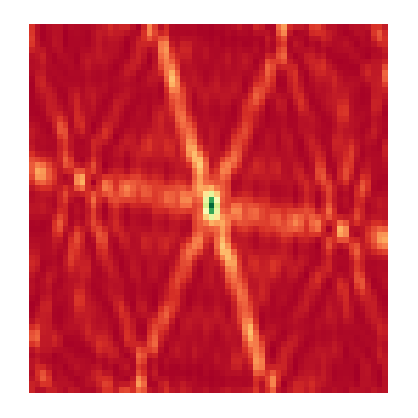
\includegraphics[width=\linewidth, trim={18px 19px 18px 18px}, clip]{./chapters/01.intro/img/psf.png}
		\caption{PSF}
	\end{subfigure}

	\begin{subfigure}[b]{0.28\linewidth}
		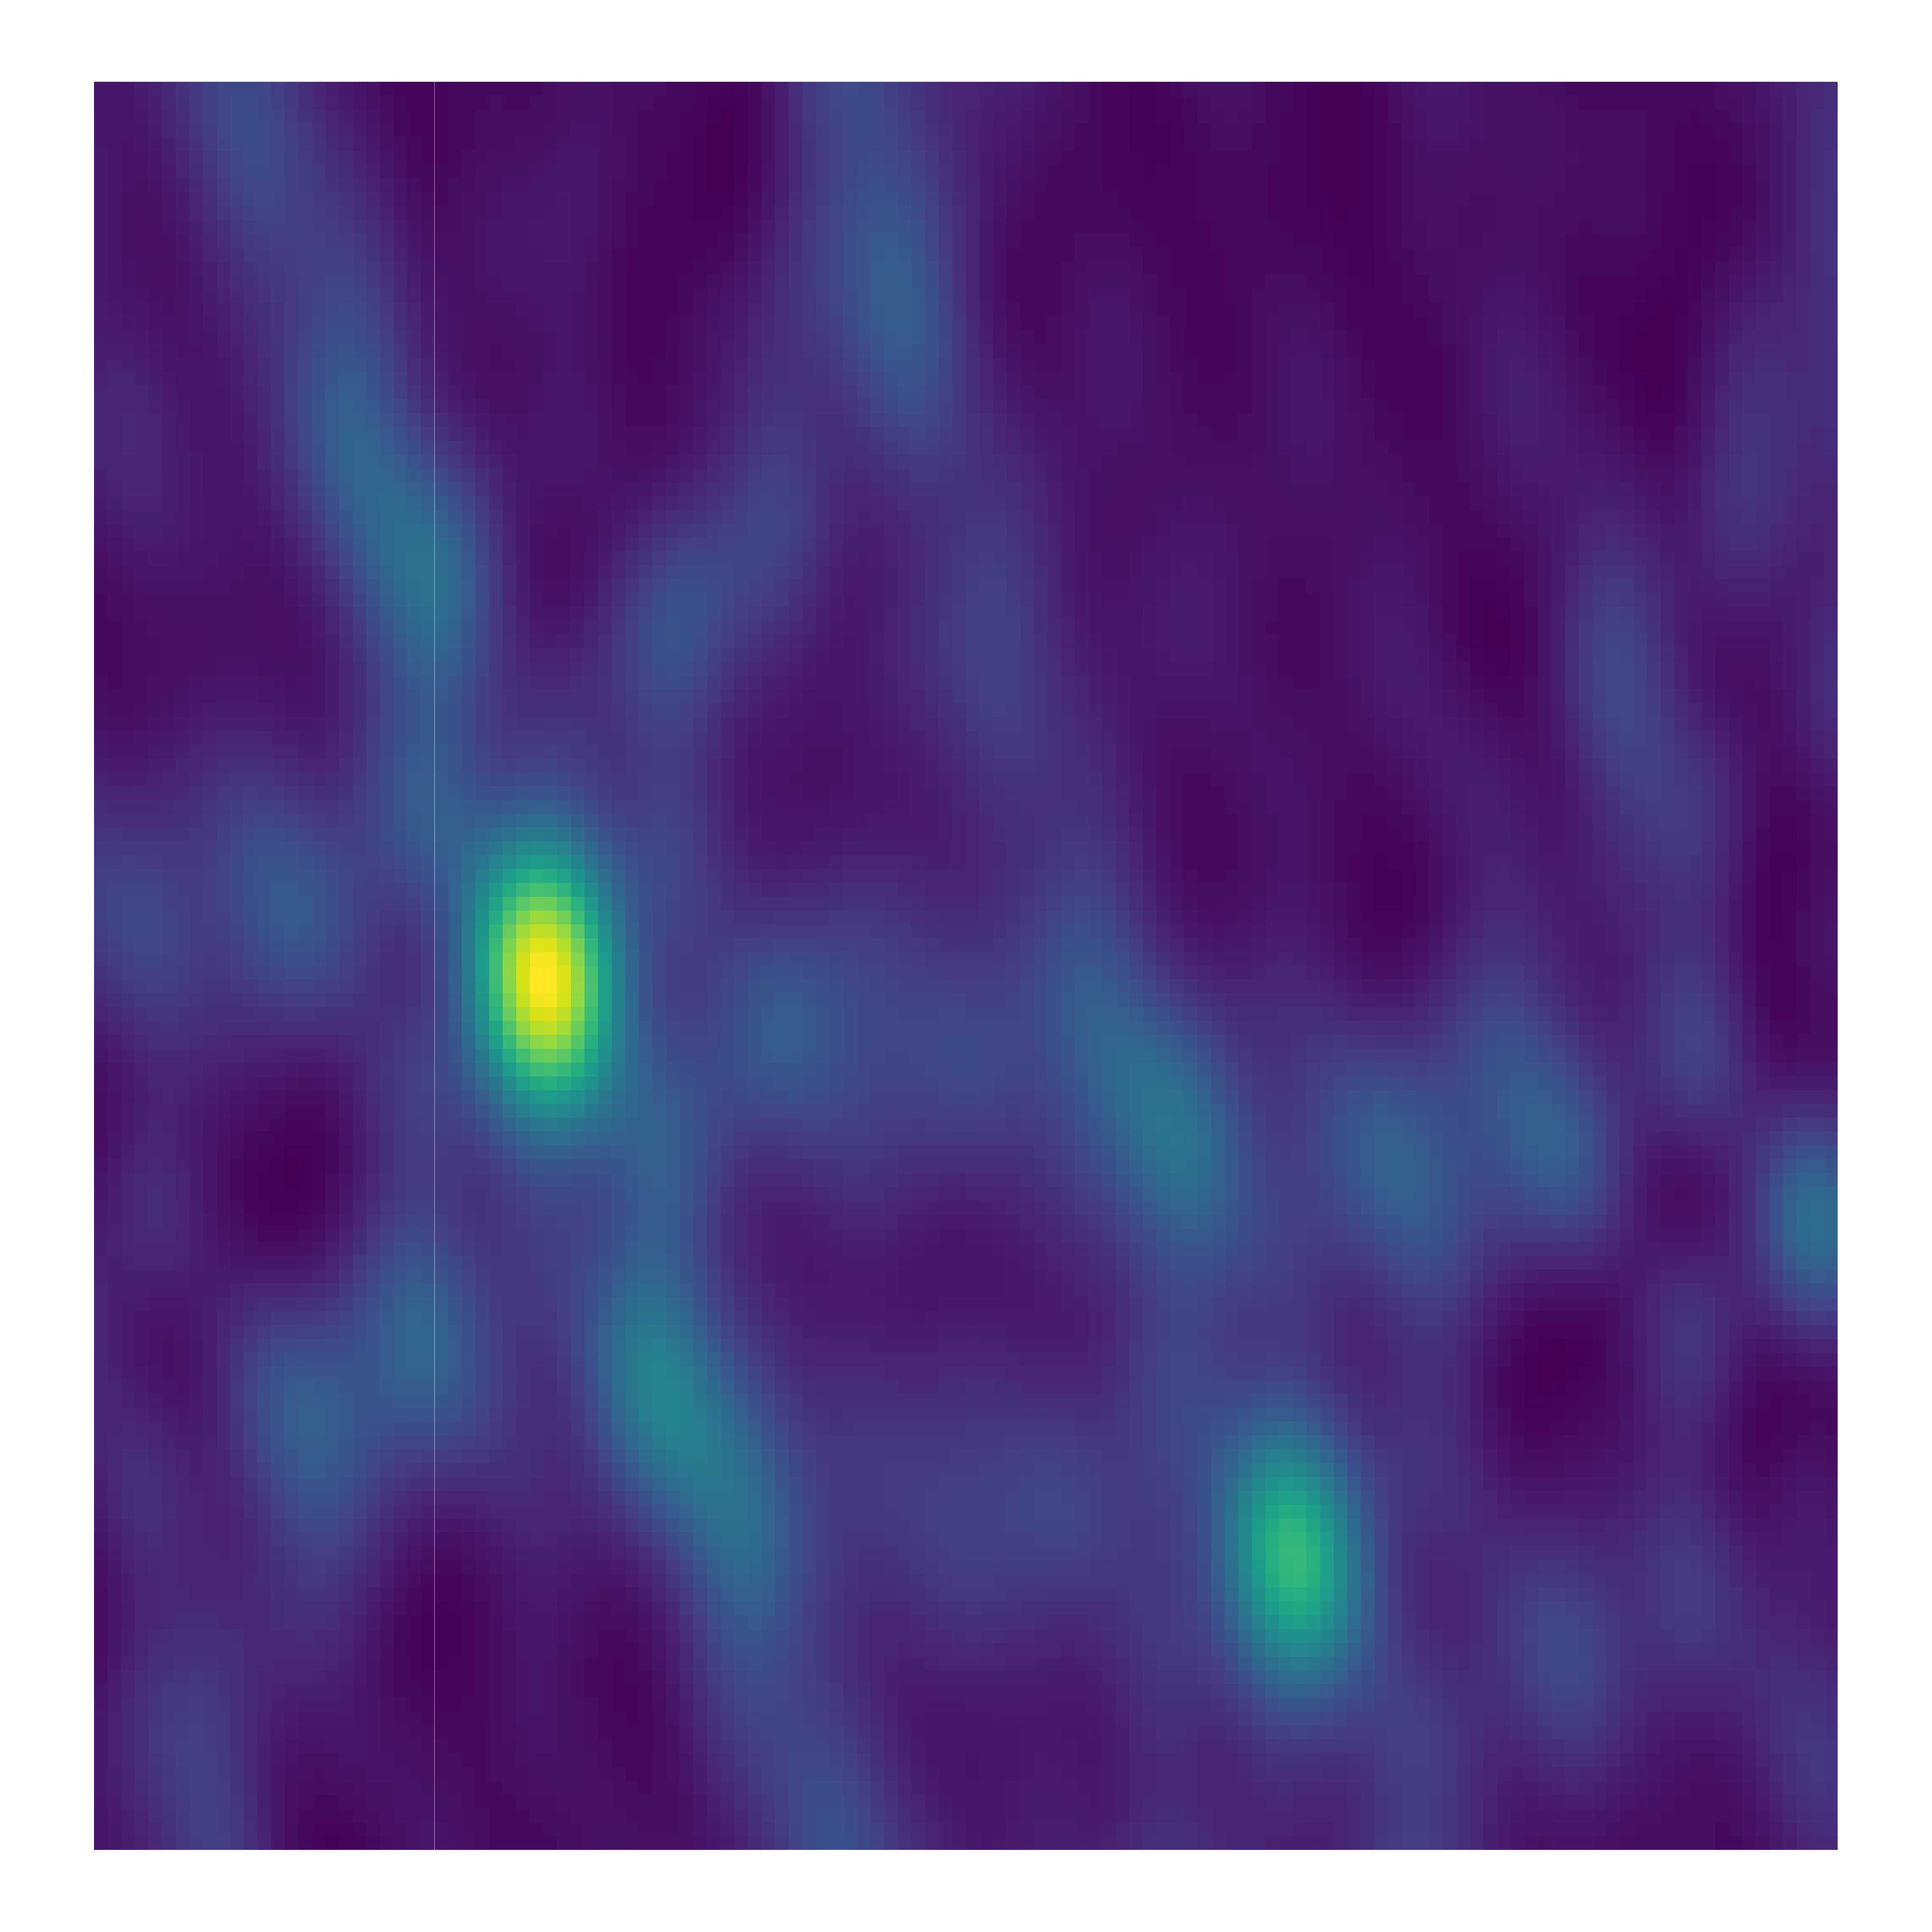
\includegraphics[width=\linewidth, trim={18px 19px 18px 18px}, clip]{./chapters/01.intro/img/dirty_image.png}
		\caption{dirty image}
	\end{subfigure}
	\begin{subfigure}[b]{0.28\linewidth}
		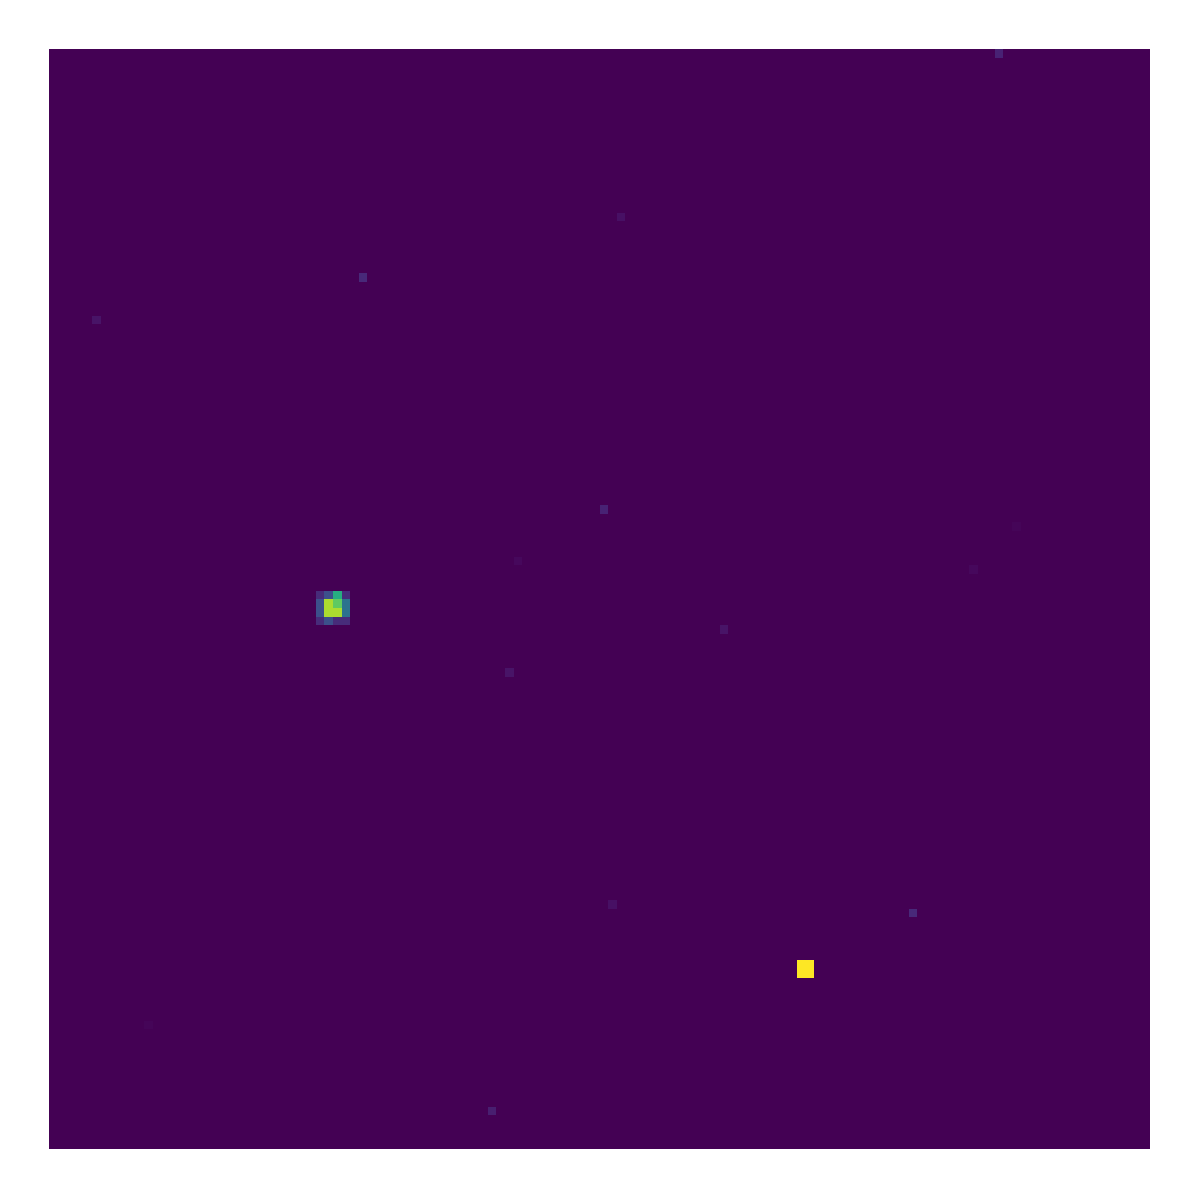
\includegraphics[width=\linewidth, trim={18px 19px 18px 18px}, clip]{./chapters/01.intro/img/true_image.png}
		\caption{true image}
	\end{subfigure}
	\caption{Inverse Problem example for VLA: Retrieve the true image when only PSF and dirty image are known}
	\label{intro:measurement_problem}
\end{figure}

The Inverse Problem is now to remove the artefacts of the interferometer and retrieve the true image. The effects of the undersampling can be modeled by a Point Spread Function (PSF). The interferometer sees the true image of the sky, but due to undersampling it gets convolved with a PSF, resulting in the dirty image.  More formally, we try to find a solution $x$ for equation \eqref{intro:eq:deconvolve}, where only the PSF and $I_{dirty}$ are known. This problem is ill-posed: it may have multiple solutions, and a small change in the $I_{dirty}$ or the PSF may result in large changes in $x$. Furthermore, the whole problem gets corrupted by noise.

\begin{equation}\label{intro:eq:deconvolve}
x \star  PSF + N = I_{dirty} 
\end{equation}

The PSF is surprisingly easy to calculate. The Fourier Transformed PSF equals the sampling pattern in UV-Space. Remember that a convolution in image space is a multiplication in Fourier. The effects of under-sampling in image space are a convolution with the PSF. In the Fourier space it is masking all components other than the measured ones. From the Antenna Configuration we can infer the masking matrix $M$ in UV-Space. Calculating the Inverse Fourier Transform of $M$ results in the PSF.


\subsection{Deconvolution with CLEAN}
In each iteration of CLEAN, it searches the highest peak of the dirty image and removing a fraction of the PSF at that point. It stops until the next highest peak is below a threshold, or if the maximum number of iterations was reached. The fraction of the PSF, threshold and number of iterations are all tunable by the user. State of the art implementations expose even more parameters. The reconstruction quality depends on the chosen parameters and require extensive user input.

%Convolved with the primary beam
CLEAN does not solve the deconvolution problem \eqref{intro:eq:deconvolve} directly. Instead, it greedily minimizes the objective \eqref{intro:eq:clean}. It is easy to see that if CLEAN minimizes the objective to zero, it has found a solution to the original deconvolution problem in a noiseless environment.

\begin{equation}\label{intro:eq:clean}
\underset{x}{minimize} \: \left \| I_{dirty} - x \star PSF \right \|_2^2
\end{equation}

Since the original problem is ill-posed, the objective \eqref{intro:eq:clean} may have several zero points. In practice, CLEAN is stopped before it reaches zero. The addition of noise can add spurious peaks in the dirty image. By stopping early, CLEAN regularizes the objective. It assumes only a limited number of point sources exist in the image. The larger the magnitude of the peak, the more likely it is to be a real point source.

In short, CLEAN does a greedy approximation of the deconvolution problem, and assumes the resulting image consists out of a few point sources. The question remains, how close the CLEAN approximation is to the true image? If the true image consists out of a few point sources, CLEAN produces a good approximation. Extended emissions however are harder for CLEAN to reproduce. The peak of extended sources is lower than that of point sources. It is harder for CLEAN to distinguish extended sources from noise.

The CLEAN regularization scheme is not ideal for extended sources. Ideally another way of regularization would be chosen for extended emissions, but the regularization is a fixed part of the CLEAN algorithm.


\subsection{From CLEAN to Compressed Sensing}
In the Compressed Sensing Framework, an approach is split into three separate parts:
\begin{itemize}
	\item An objective with a data and regularization term.
	\item A prior $P$ in which transforms the image into a sparse domain.
	\item An optimization algorithm that is suited for the objective.
\end{itemize}

To demonstrate the flexibility of the Compressed Sensing Framework, we convert CLEAN into a Compressed Sensing approach. First we add a regularization term to \eqref{intro:eq:clean} and arrive at the new objective \eqref{intro:eq:csclean}. The objective contains the original CLEAN data term and a new regularization term. The data term forces the reconstruction to be close to the measurement, while the regularization term forces the reconstruction to be plausible. $\lambda$ models the expected noise in the problem. Note that the $\left \| Px \right \|_0$ acts as an indicator function. 

\begin{equation}\label{intro:eq:csclean}
	\underset{x}{minimize} \: \left \| D_{dirty} - x \star PSF \right \|_2^2 \: + \: \lambda \left \| Px \right \|_0
\end{equation}

The Prior $P$ transforms the image in a sparse domain. CLEAN assumes the $x$ contains a few point sources. In Compressed Sensing terminology, it assumes $x$ is sparse in image space. Since $x$ is already an image, the Prior $P$ in Compressed Sensing CLEAN is the identity matrix.  

The last step is choosing a similar optimization algorithm: In every iteration, CLEAN searches the highest peak in the dirty image. Matching Pursuit is a greedy optimization algorithm. In every iteration it searches the step which minimizes \eqref{intro:eq:csclean} the most.


Same as clean, but now we have a global optimization scheme. The CLEAN parameters are not needed any more, $\lambda$ can be estimated. Different parts can be replaced: $P$ can be replaced with Total Variation Prior, Wavelet Transform or Starlets without changing the objective function or the optimization algorithm. 

A lot of freedom to design, which is why it is interesting for wide Field of View imaging. active field of research. Interest because it can solve the three problems in Radio Astronomy:
Model the effects of wide Field of View imaging.
Model the true image and improve the reconstruction for extended sources.
Scalable optimization algorithm to handle the data of new large interferometers.



\newpage
\section{Inverse Problem for wide Field of View Imaging} \label{radio}
So far the small Field of View inverse problem has been introduced where each antenna pair measures a Visibility of the sky brightness distribution. This leads to the small Field of View measurement equation \eqref{radio:eq:2dft}. It is identical to the two dimensional Fourier Transform. In practice the Fast Fourier Transform is used which scales better on large problems.

\begin{equation}\label{radio:eq:2dft}
V(u, v) = \int\int x(l, m) e^{2 \pi i (ux+vy)} dl dm
\end{equation}

For wide Field of View imaging, two effects break the two dimensional Fourier Transform relationship: Non-coplanar Baselines and the celestial sphere which lead to the measurement equation \eqref{radio:eq:ftSphere}. Note that for small Field of View $1 - x^2 -y ^2 \ll 1$, and \eqref{radio:eq:ftSphere} reduces to the 2d measurement equation \eqref{radio:eq:2dft}. 

\begin{equation}\label{radio:eq:ftSphere}
	V(u, v, w) = \int\int \frac{X(x, y)}{\sqrt{1 - x^2 - y ^2}} e^{2 \pi i (ux+vy+ w\sqrt{1 - x^2 - y ^2})}dx dy
\end{equation}

\begin{wrapfigure}{r}{0.5\textwidth}
	\centering
	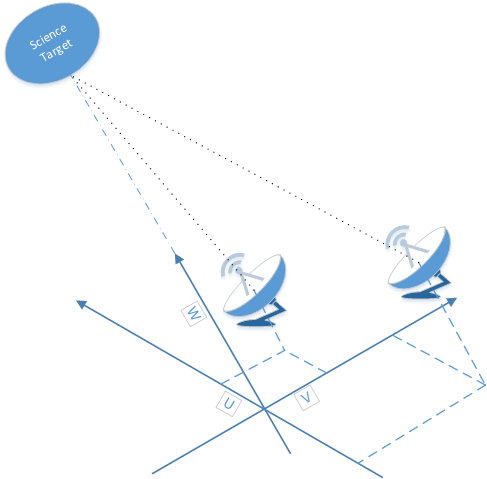
\includegraphics[width=0.9\linewidth]{./chapters/03.radio/uvw.png}
	\caption{U V and W coordinate space}
	\label{radio:uvw}
	\vspace{-10pt}
\end{wrapfigure}

Non-coplanar Baselines lead to a third component $w$ for each Visibility. Figure \ref{radio:uvw} shows the the $u$ $v$ and $w$ coordinate system. $w$ is essentially the pointing direction of the instrument. The UV-Plane is the projection of the antennas on a plane perpendicular to the pointing direction. Which point in the UV-Plane get sampled and what $w$ component it has depends on the pointing direction. If the instrument points straight up, the UV-Plane is a tangent to earth's surface, and the $w$ term compensates for earth's surface curvature. If however the instrument points at the horizon, the projected UV-Plane gets squashed and $w$ compensates for antennas which lie far behind the UV-Plane. In essence, $w$ is a phase delay that corrects antenna positions in three dimensions. The wide Field of View measurement equation \eqref{radio:eq:ftSphere} would account for the $w$ phase delay, but it breaks the the two dimensional Fourier relationship and the FFT cannot be used. The W-Projection \cite{cornwell2008noncoplanar} algorithm approximates the effect of the $w$ term restores the two dimensional Fourier relationship.



Non-coplanar baselines, each Visibility has a $u$ and $v$ component. $u$ and $v$ are vectors on a plain. The plains normal points to the science target. 
So far the simplified inverse problem has been introduced. Each antenna pair measures a Fourier Component of the sky brightness distribution. The distance between antenna pairs dictates what point is sampled in the UV plane. This leads to the measurement equation . Calculating the true image $X$ is simply inverting the two dimensional Fourier Transform.

In reality, each visibility has a third component $w$. It comes from the fact that the antennas are not on a flat plane but on the curved surface of the earth. Image  shows the three dimensional space. $w$ is the vector points from the phase center to the science target. For small Field of Views, the effect is negligible and the measurement equation \eqref{radio:eq:2dft} is a good approximation. The field of view is limited by the primary beam of the antennas. Primary beam widens with wavelength. So far, wide Field of View problems were encountered in low frequencies like LOFAR.


new instruments like SKA, ASKAP and Pathfinder are constructed with a wide Field of View in mind. The simple two dimensional Fourier Transform does not hold true anymore and we arrive at the wide Field of View measurement equation \eqref{radio:eq:ftSphere}.


 can be approximated by the 2d Fourier Transform \eqref{radio:eq:2dft}. Two separate effects: $w$ Component for non coplanar baselines.



A-Projection \cite{tasse2013applying}

spread spectrum phenomenon

All here to try to get back to the 2d fourier transform. 

%"The field of view of a telescope is limited by the primary beams of the antennas. To map a region of sky where the emission is at a scale larger than the angular width of the primary beams, mosaicing needs to be done. This is discussed in the second part of this lecture."

%Phase 

%source \cite{lfraSchool}


Strength of compressed sensing is modelling these effects.

\subsection{Calibration}
A lot of effects, weather, noise, antenna temperature, drift.

Antenna based calibration, holds true for current interferometers but is not true for SKA. Possible switch to baseline based calibration.

\subsubsection{Self-Calibration}
?
\newpage
\section{Sparsity and Compressed Sensing}

\begin{equation}\label{intro:underdetermined}
\begin{split}
Fx = y
\end{split}
\begin{split}
x &\in \mathcal{R}^n\\
y &\in \mathcal{C}^m\\
2m &< n
\end{split}
\end{equation}

\section{The Theory of Compressed Sensing} \label{cs}
If we have a bandwidth-limited Signal, how many samples do we need to reconstruct it? The Nyquist-Shannon Sampling Theory states if we have equidistant samples, our sampling rate needs to be more than twice the highest frequency component of the signal. If the sampling rate is lower, the reconstructed signals will be subject to aliasing, it will be different from the reality. However, Compressed Sensing is able to 

Compressible Signals, Sparsity


Compressible Signals, finding the true solution

\subsection{Compressible Signals and Priors}


\subsection{Compressed Sensing Algorithms in Radiointerferometry}

\subsection{Modelling}

\subsection{Implementation In Casa}

\subsubsection{The Major and Minor Cycle}

\newpage
\section{Reconstruction of Supernova Remnant G55} \label{results}

\begin{figure}[h]
	\centering
	\begin{subfigure}[b]{0.45\linewidth}
		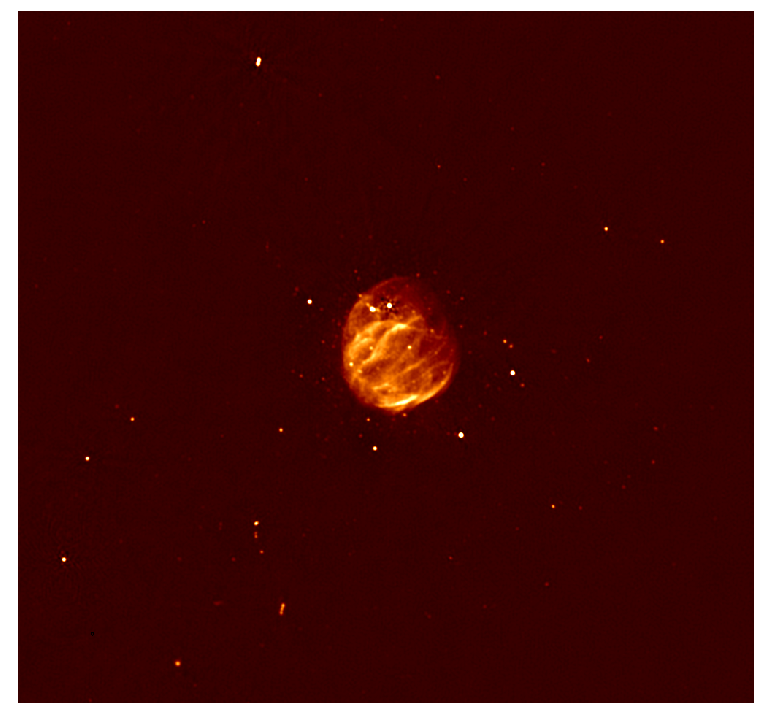
\includegraphics[width=\linewidth, trim={230px 210px 225px 200px}, clip]{./chapters/05.results/pic_G55_7.png}
		\caption{Reconstruction by NRAO.  Source:\cite{nraoG55}}
		\label{results:g55:nrao:rec}
	\end{subfigure}
	\begin{subfigure}[b]{0.45\linewidth}
		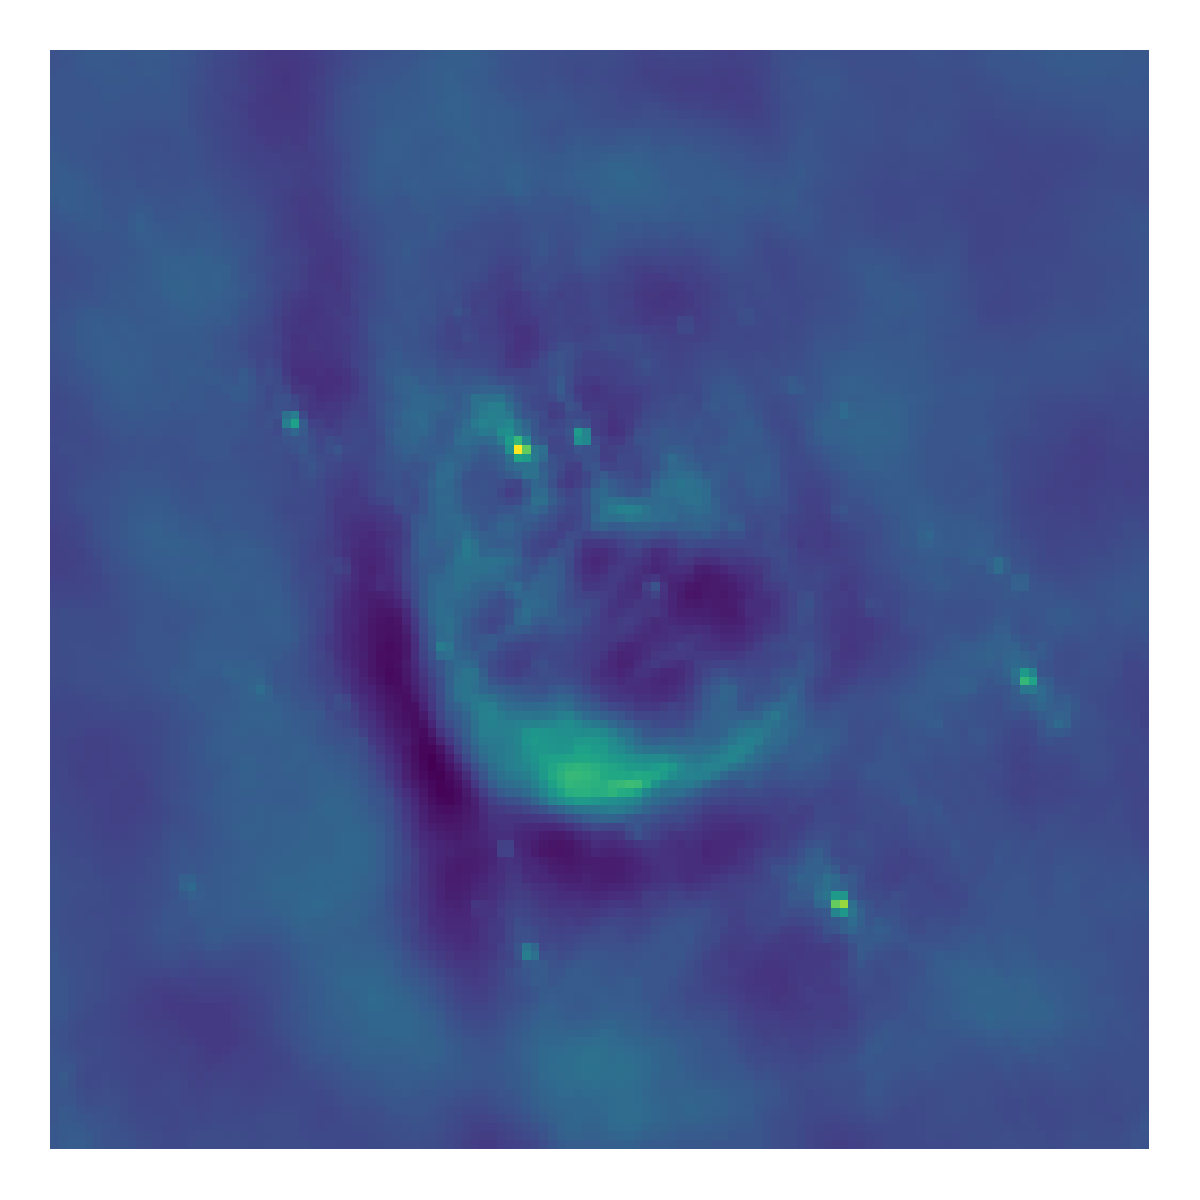
\includegraphics[width=\linewidth, trim={18px 19px 18px 18px}, clip]{./chapters/05.results/g55/raw_image.png}
		\caption{Dirty Image}
		\label{results:g55:nrao:dirty}
	\end{subfigure}
	\caption{SNR G55 source observed by VLA.}
	\label{results:g55:nrao}
\end{figure}

The supernova remnant (SNR) G55 was observed by VLA. 10 seconds of the 8 hour observation is publicly available through the CASA imaging tutorial\cite{casaImagingGuide}. \ref{results:g55:nrao:dirty} is the dirty image calculated from the 10 second observation. The full 8 hours are not readily available. The image \ref{results:g55:nrao:rec} is a reconstruction from an unknown VLA observation. The deconvolution algorithm is also unknown. For this project, the image \ref{results:g55:nrao:rec} is assumed to show the true image of the sky.

The image \ref{results:g55:nrao:rec} shows G55 to be a slightly "egg shaped" extended emission with six strong point sources. Several fainter point sources are inside and around the egg shaped extended emission. The dirty image \ref{results:g55:nrao:dirty} shows a corrupted version of G55. The six strong point sources are clearly visible as are the brighter parts of the extended emission. The dirty image also shows a negative "trench" striking through the image as well as brighter regions around the remnant. 

The images in figure \ref{results:g55:nrao} spans a size of 55 arc-minutes. For small field of view imaging, images with half the size are usually the limit. In the real world, wide field imaging would be used. In this project, small field of view imaging was used because it is quicker to compute. It limits the dynamic range of the dirty image, the whole task gets harder for the reconstruction algorithm.

The CLEAN algorithm gets compared to Compressed Sensing Reconstructions. The parameters of CLEAN were taken from the CASA imaging tutorial\cite{casaImagingGuide}. The reconstructed images of Compressed Sensing are constrained to have no negative pixels. Negative pixels are not physically plausible and was shown to improve Compressed Sensing reconstructions for synthetic data\cite{mcewen2011compressed}. In total six different priors were tested with the analysis objective:
\begin{enumerate}
	\item No Regularization
	\item L1
	\item L2
	\item L1+L2
	\item Total Variation
	\item Starlet Transform
\end{enumerate}

To reduce the memory requirements, the PSF was truncated. Any value smaller than 0.02 of the PSF was truncated to zero. The current implementation requires a quadratic amount of memory per pixel. The images here have a size of $128*128$ pixels, which was the maximum for current desktop machines.

The regularization parameter $\lambda$ needs to be estimated for each prior. The Miller\cite{miller1970least} $\lambda$ estimation was used and is shown in equation \eqref{results:eq:miller}. An approximate solution is needed for the bounds $e$ and $E$. In this project, the result with no regularization was used for the $\lambda$ estimation. For practical applications the image effectively gets reconstructed twice. Other Compressed Sensing Reconstructions approximate $x$ of equation \eqref{results:eq:miller} by running their optimizer a fixed number of iterations without regularization, which reduces the computational costs.

\begin{equation}\label{results:eq:miller}
	\lambda = e / E \qquad  \left \| I_{dirty} - x \star PSF \right \|_2^2 \le e \qquad p(x) \le E
\end{equation}

Two figures compare the Dirty Image, CLEAN and the Compressed Sensing Reconstrutions. Figure \ref{res:g55:img} shows the reconstructed images on the same intensity scale. Figure \ref{res:g55:profile} shows the flux profile of the reconstructed images.

\begin{figure}[h!]
	\centering
	\begin{subfigure}[b]{0.32\linewidth}
		\centering{Dirty Image}
		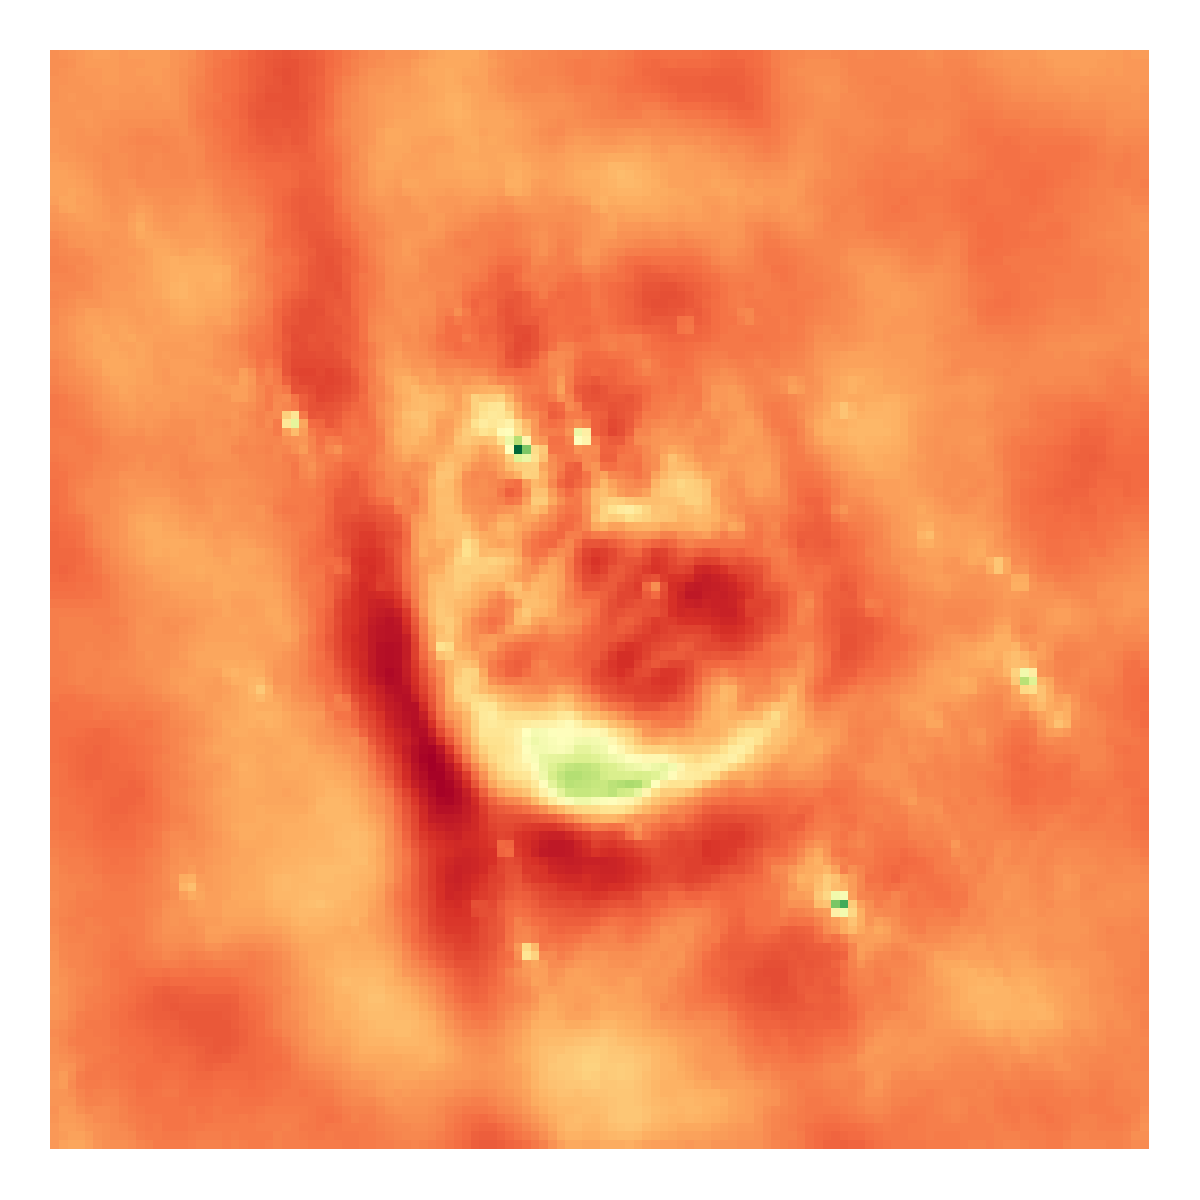
\includegraphics[width=\linewidth, trim={20px 30px 75px 52px}, clip]{./chapters/05.results/g55/raw_model.png}
	\end{subfigure}
	\begin{subfigure}[b]{0.32\linewidth}
		\centering{CLEAN}
		
\includegraphics[width=\linewidth, trim={20px 30px 75px 52px}, clip]{./chapters/05.results/g55/clean_model.png}
	\end{subfigure}
	\begin{subfigure}[b]{0.32\linewidth}
		\centering{No Regularization}
		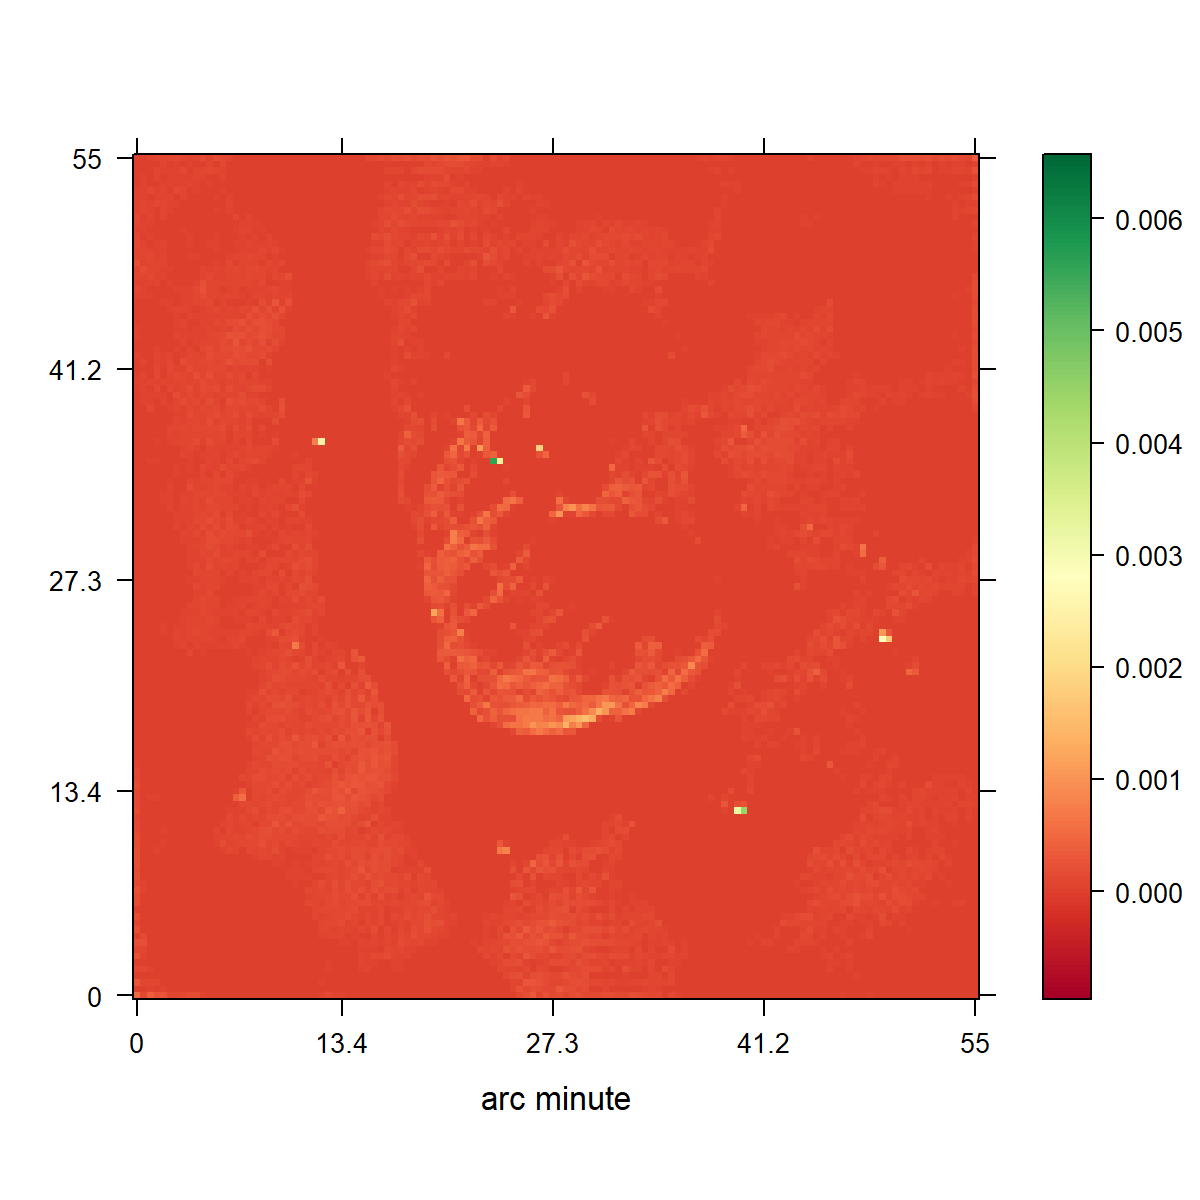
\includegraphics[width=\linewidth, trim={20px 30px 75px 52px}, clip]{./chapters/05.results/g55/positive_deconv_model.png}
	\end{subfigure}

	\begin{subfigure}[b]{0.32\linewidth}
		\centering{L1}
		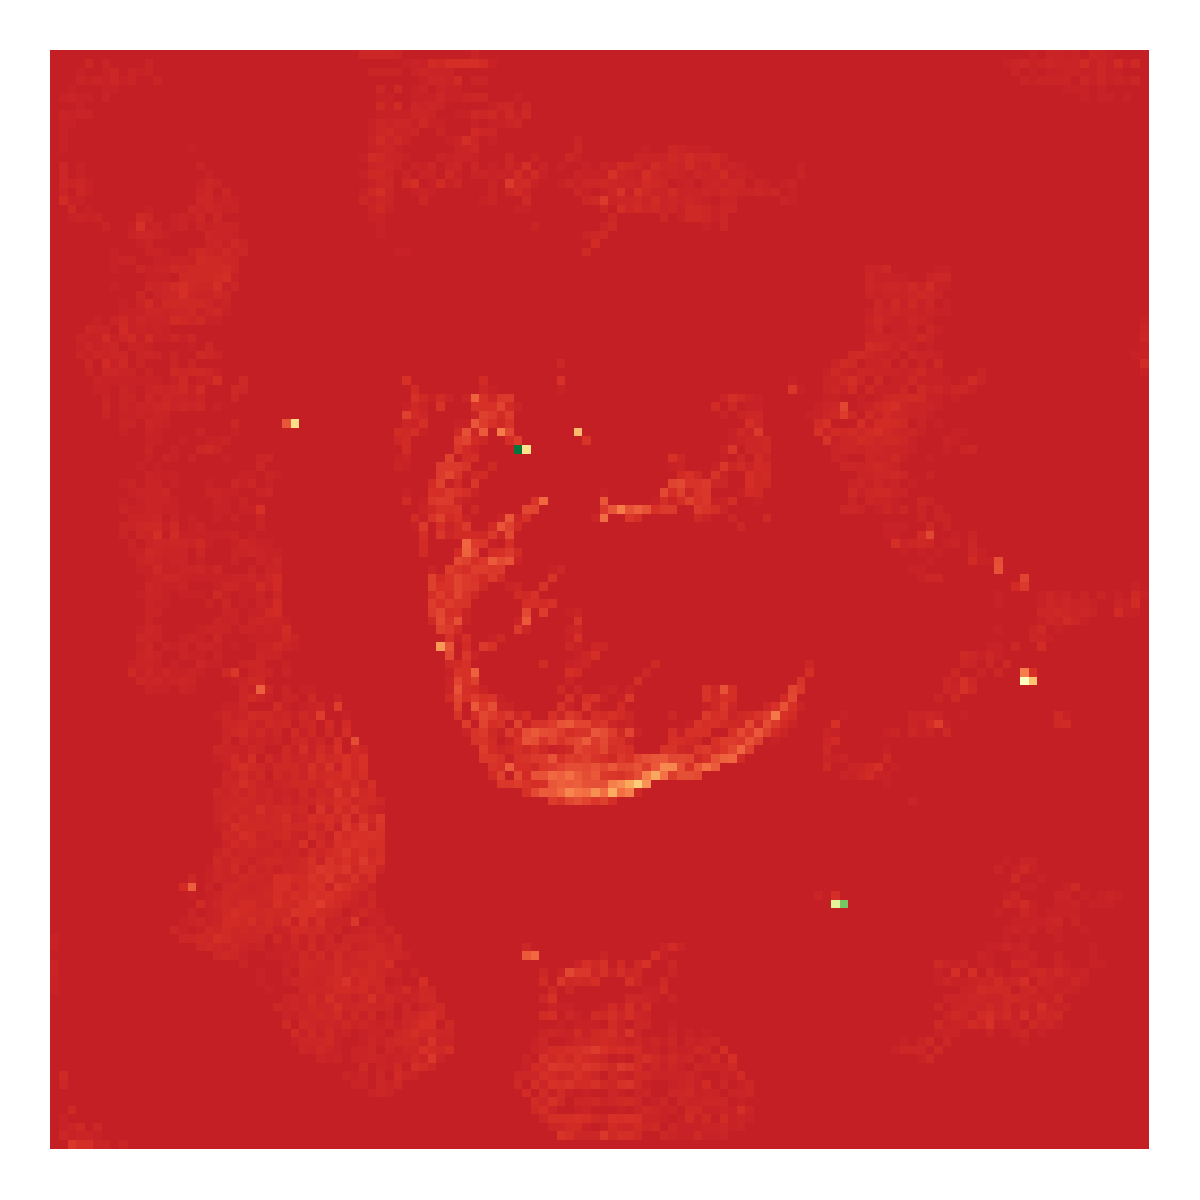
\includegraphics[width=\linewidth, trim={20px 50px 75px 52px}, clip]{./chapters/05.results/g55/L1_model.png}
	\end{subfigure}
	\begin{subfigure}[b]{0.32\linewidth}
		\vspace{10pt}
		\centering{L2}
		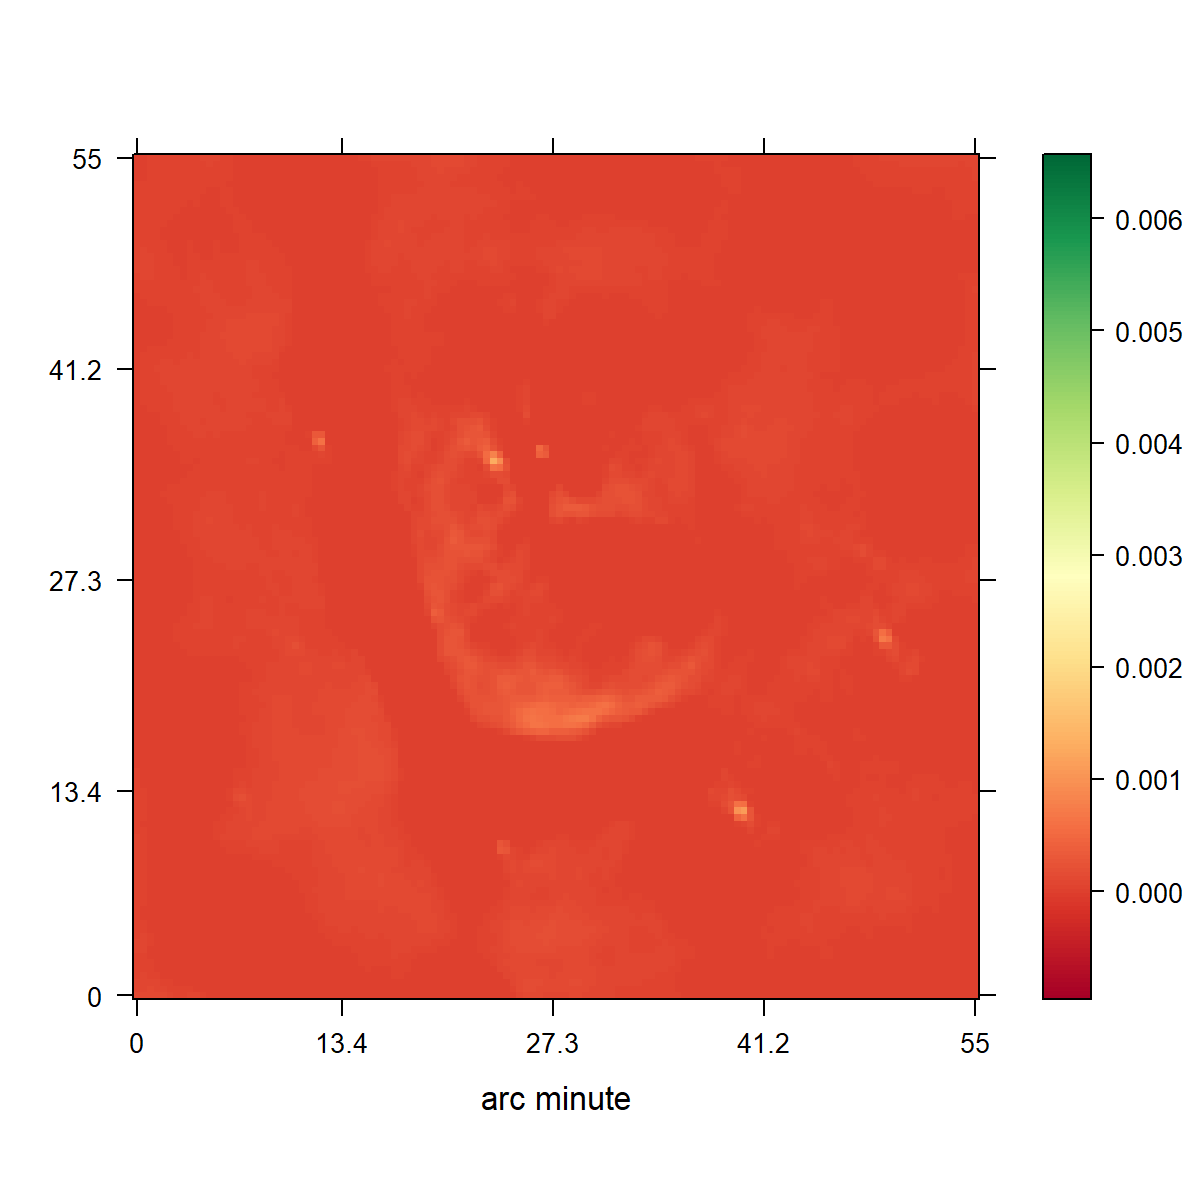
\includegraphics[width=\linewidth, trim={20px 50px 75px 52px}, clip]{./chapters/05.results/g55/L2_model.png}
	\end{subfigure}
	\begin{subfigure}[b]{0.32\linewidth}
		\centering{L1+L2}
		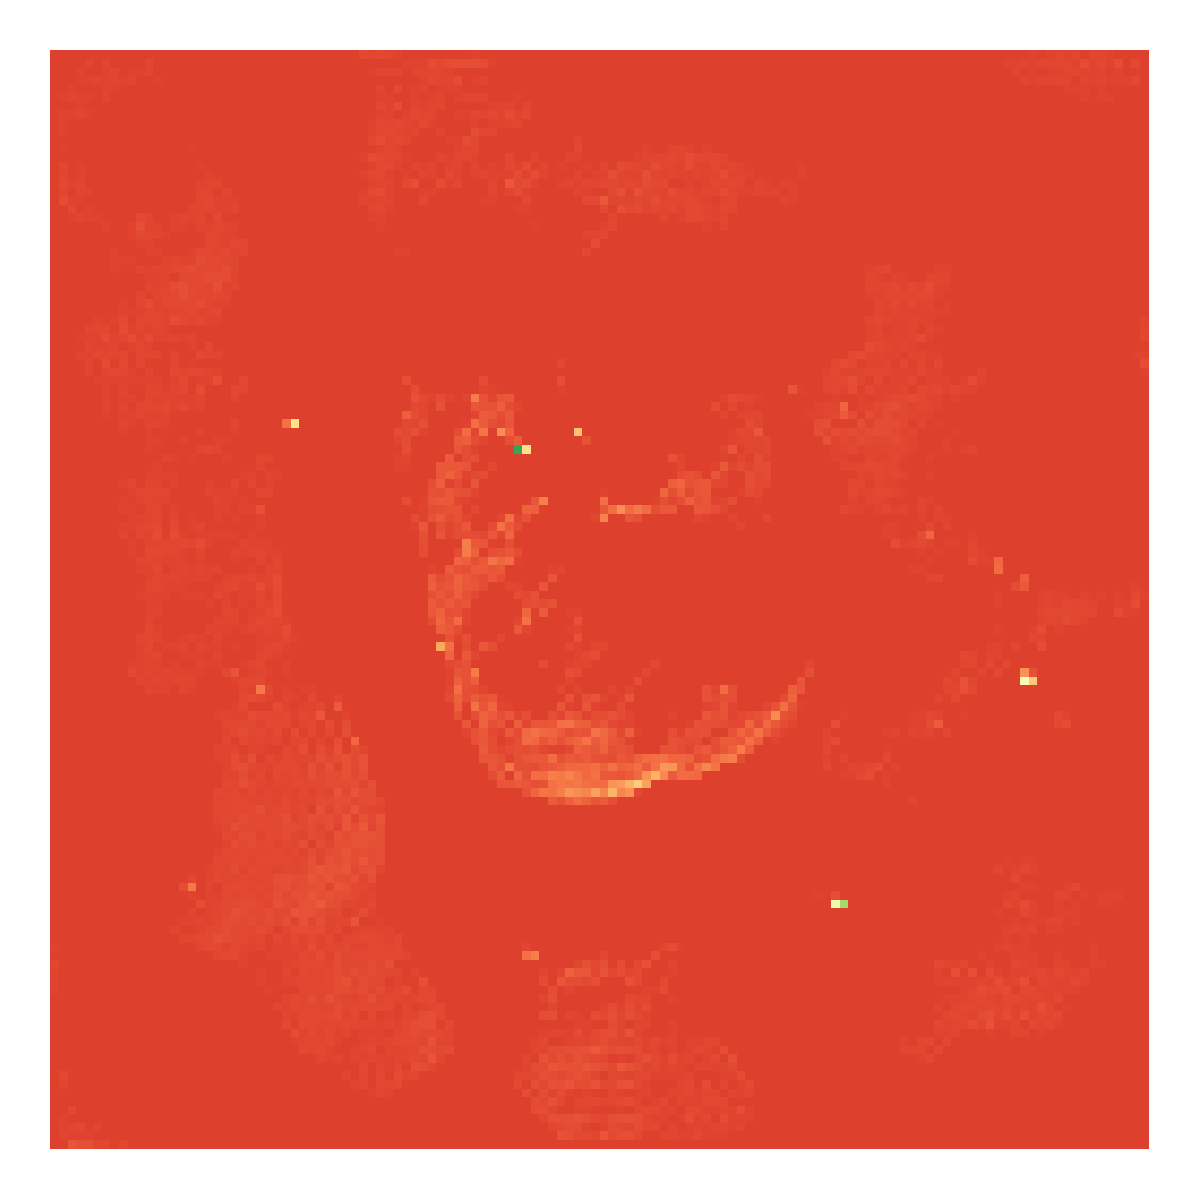
\includegraphics[width=\linewidth, trim={20px 50px 75px 52px}, clip]{./chapters/05.results/g55/L1+L2_model.png}
	\end{subfigure}

	\begin{subfigure}[b]{0.32\linewidth}
		\vspace{10pt}
		\centering{Total Variation}
		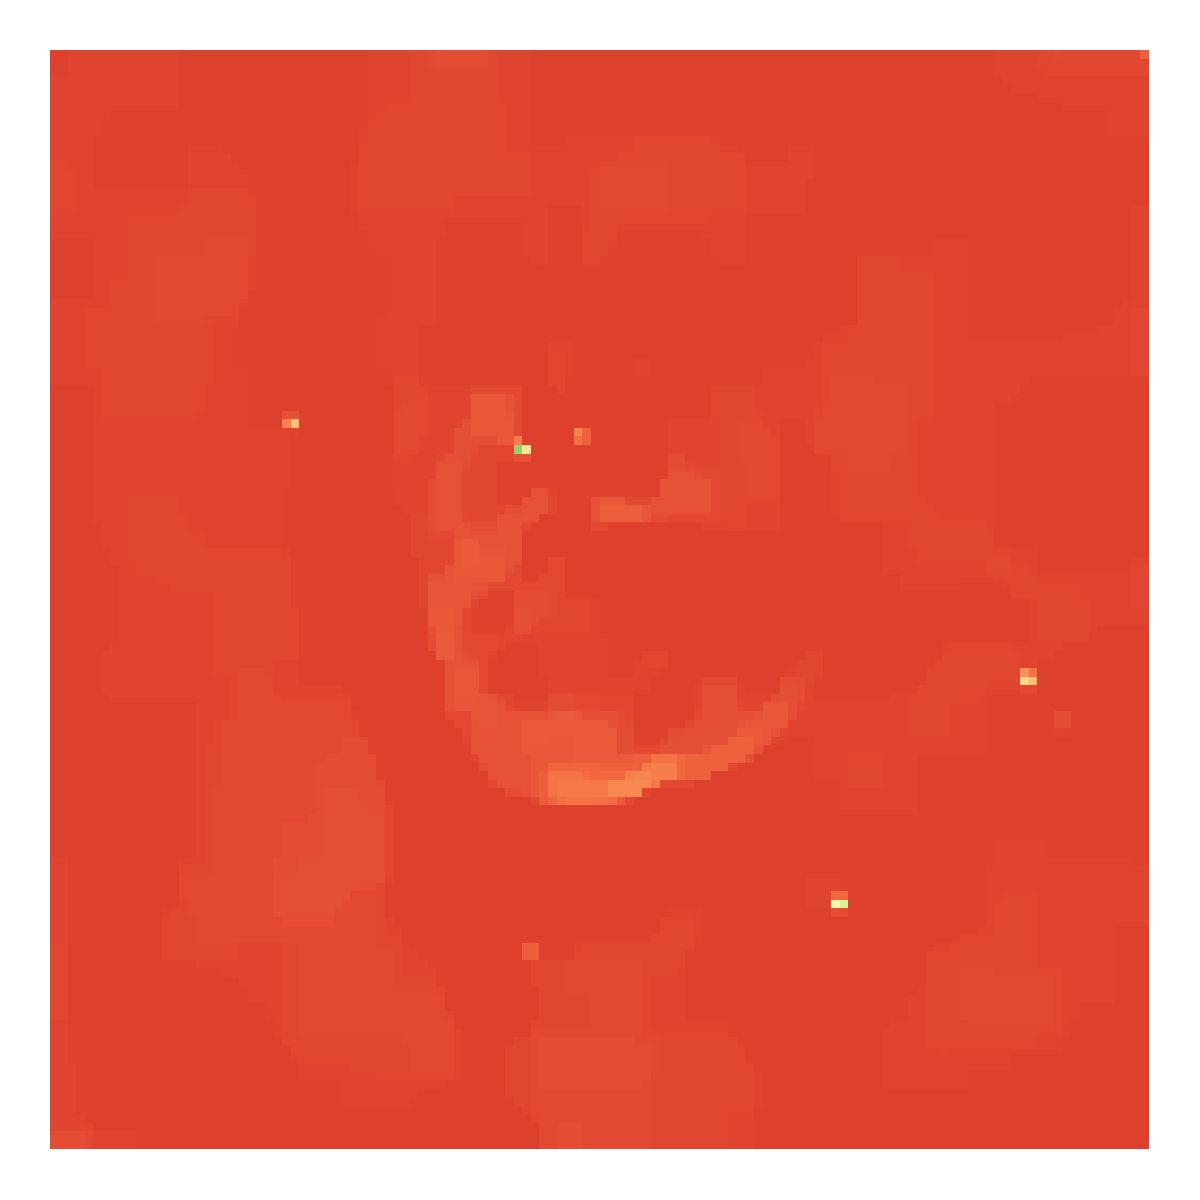
\includegraphics[width=\linewidth, trim={20px 50px 75px 52px}, clip]{./chapters/05.results/g55/TV_model.png}
	\end{subfigure}
	\begin{subfigure}[b]{0.392\linewidth}
		\centering{Starlets}
		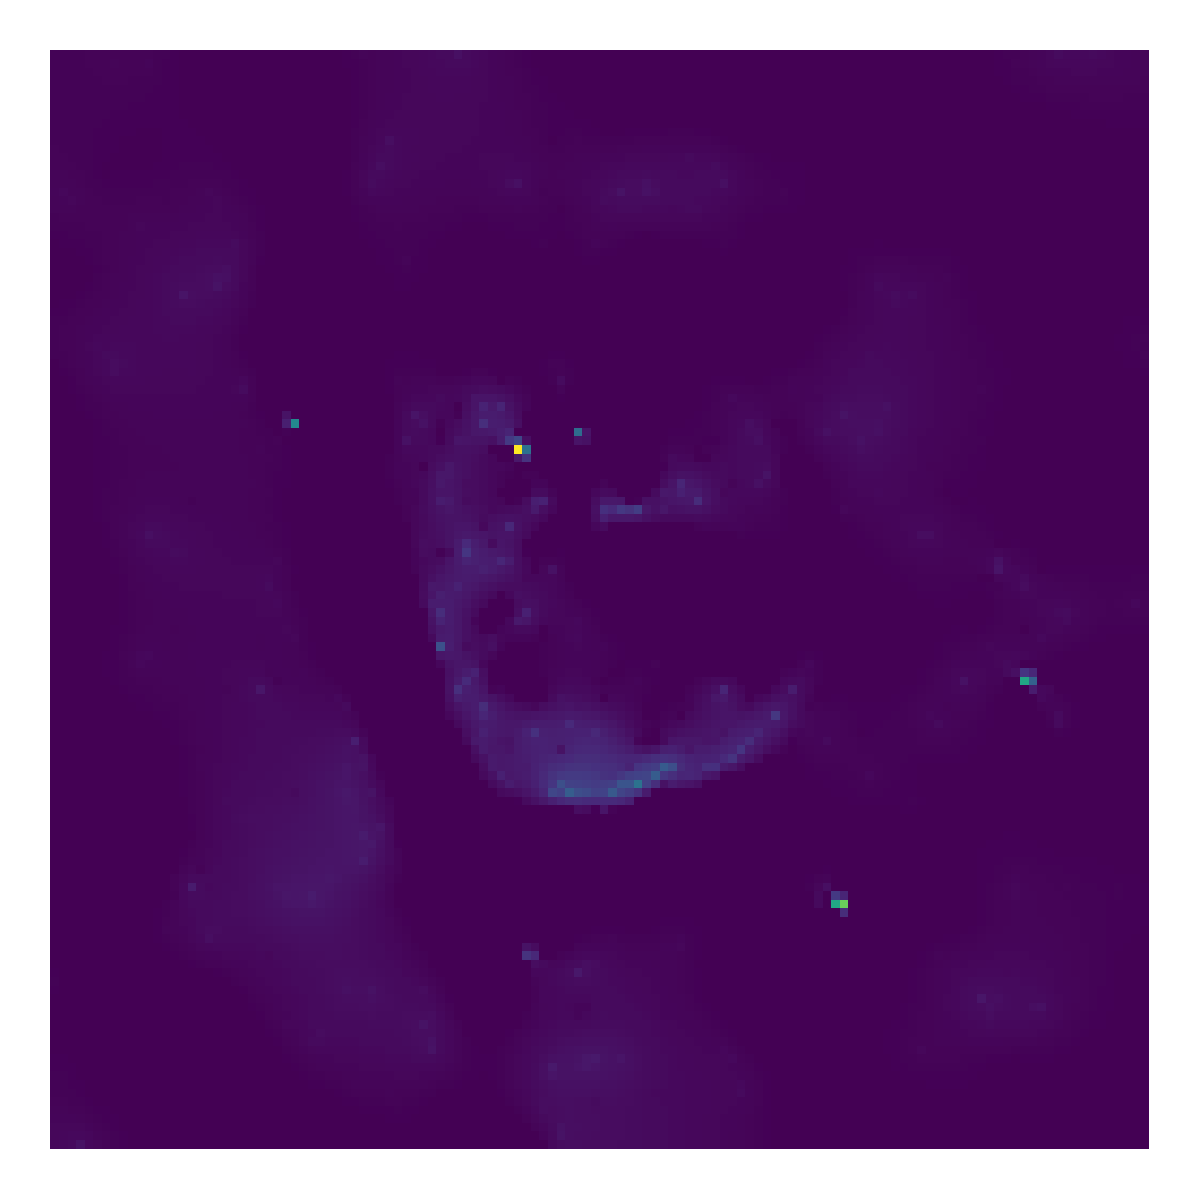
\includegraphics[width=\linewidth, trim={20px 50px 0px 52px}, clip]{./chapters/05.results/g55/starlets3_model.png}
	\end{subfigure}
	\caption{Reconstructed images of CLEAN and the different Compressed Sensing priors.} 
	\label{res:g55:img}
\end{figure}

\begin{figure}
	\centering
	\begin{subfigure}[b]{0.9\linewidth}
		\centering
		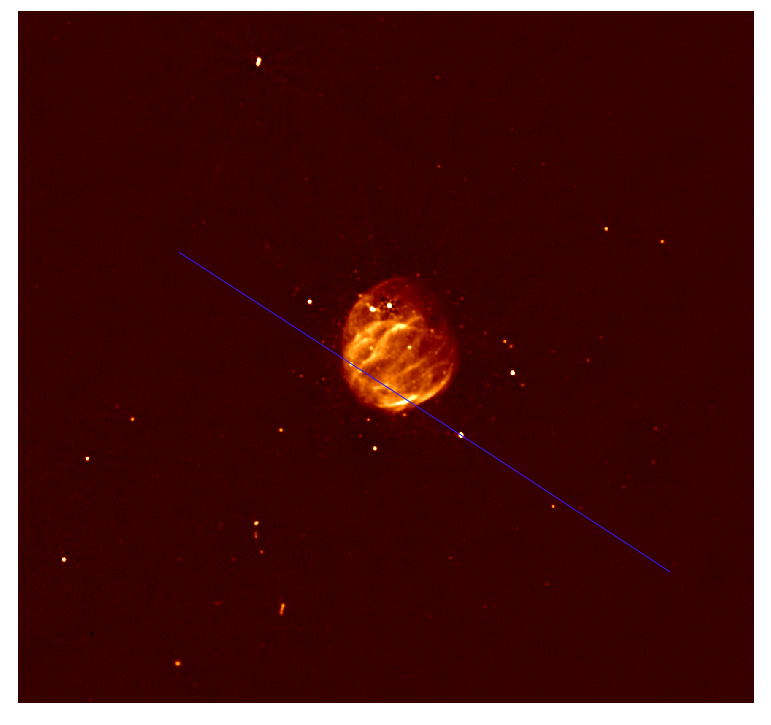
\includegraphics[width=0.3\linewidth, trim={180px 170px 170px 146px}, clip]{./chapters/05.results/pic_G55_7_lined.png}
		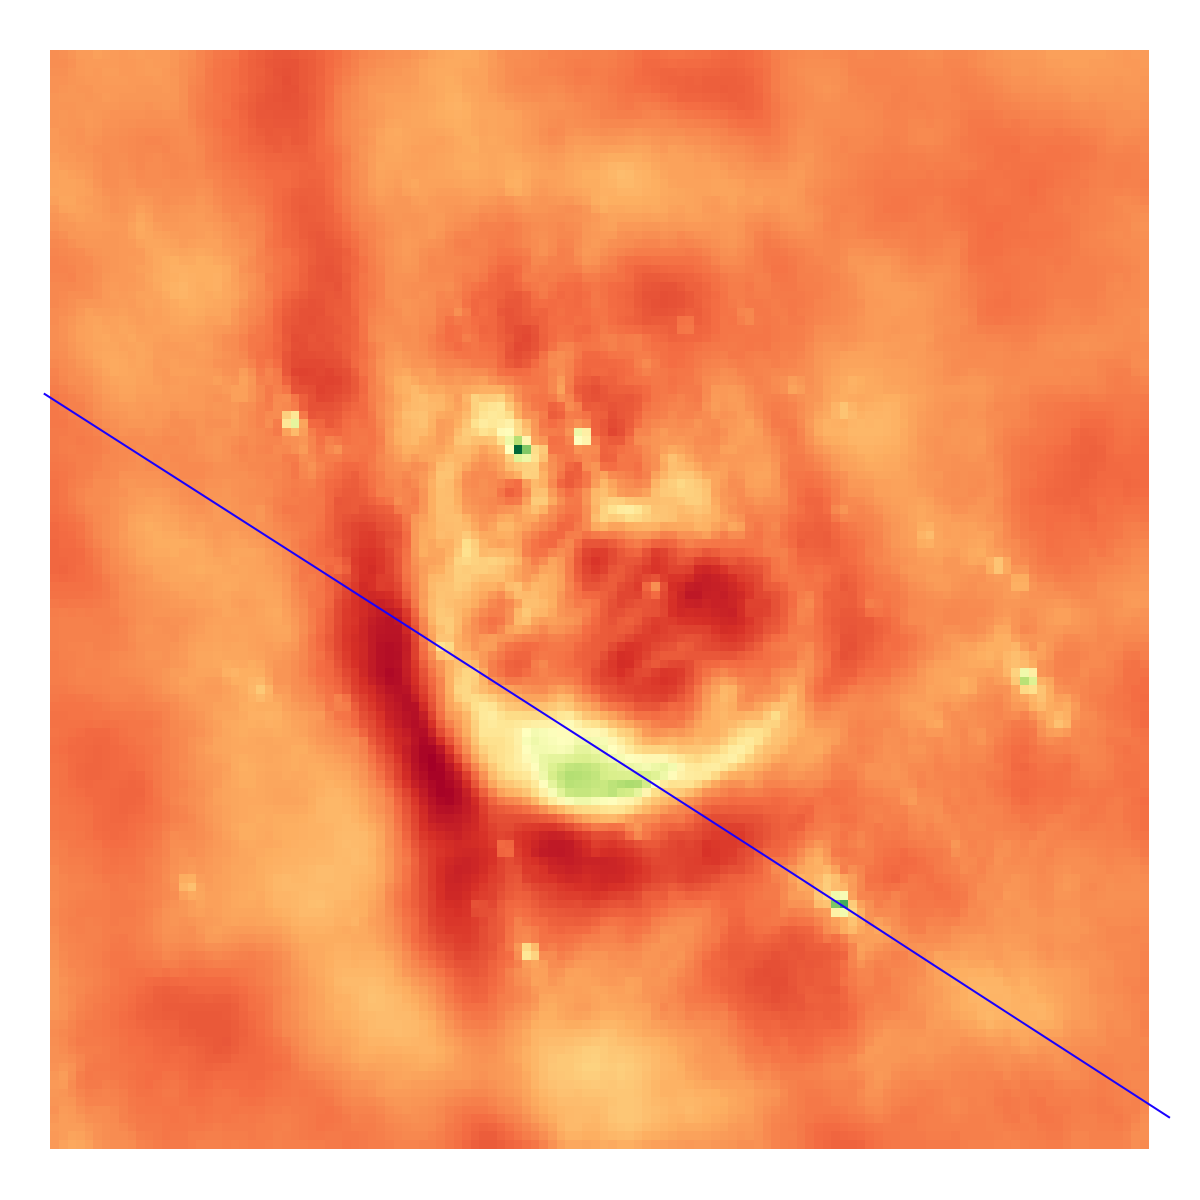
\includegraphics[width=0.3\linewidth, trim={18px 19px 18px 18px}, clip]{./chapters/05.results/raw_image_lined.png}
	\end{subfigure}

	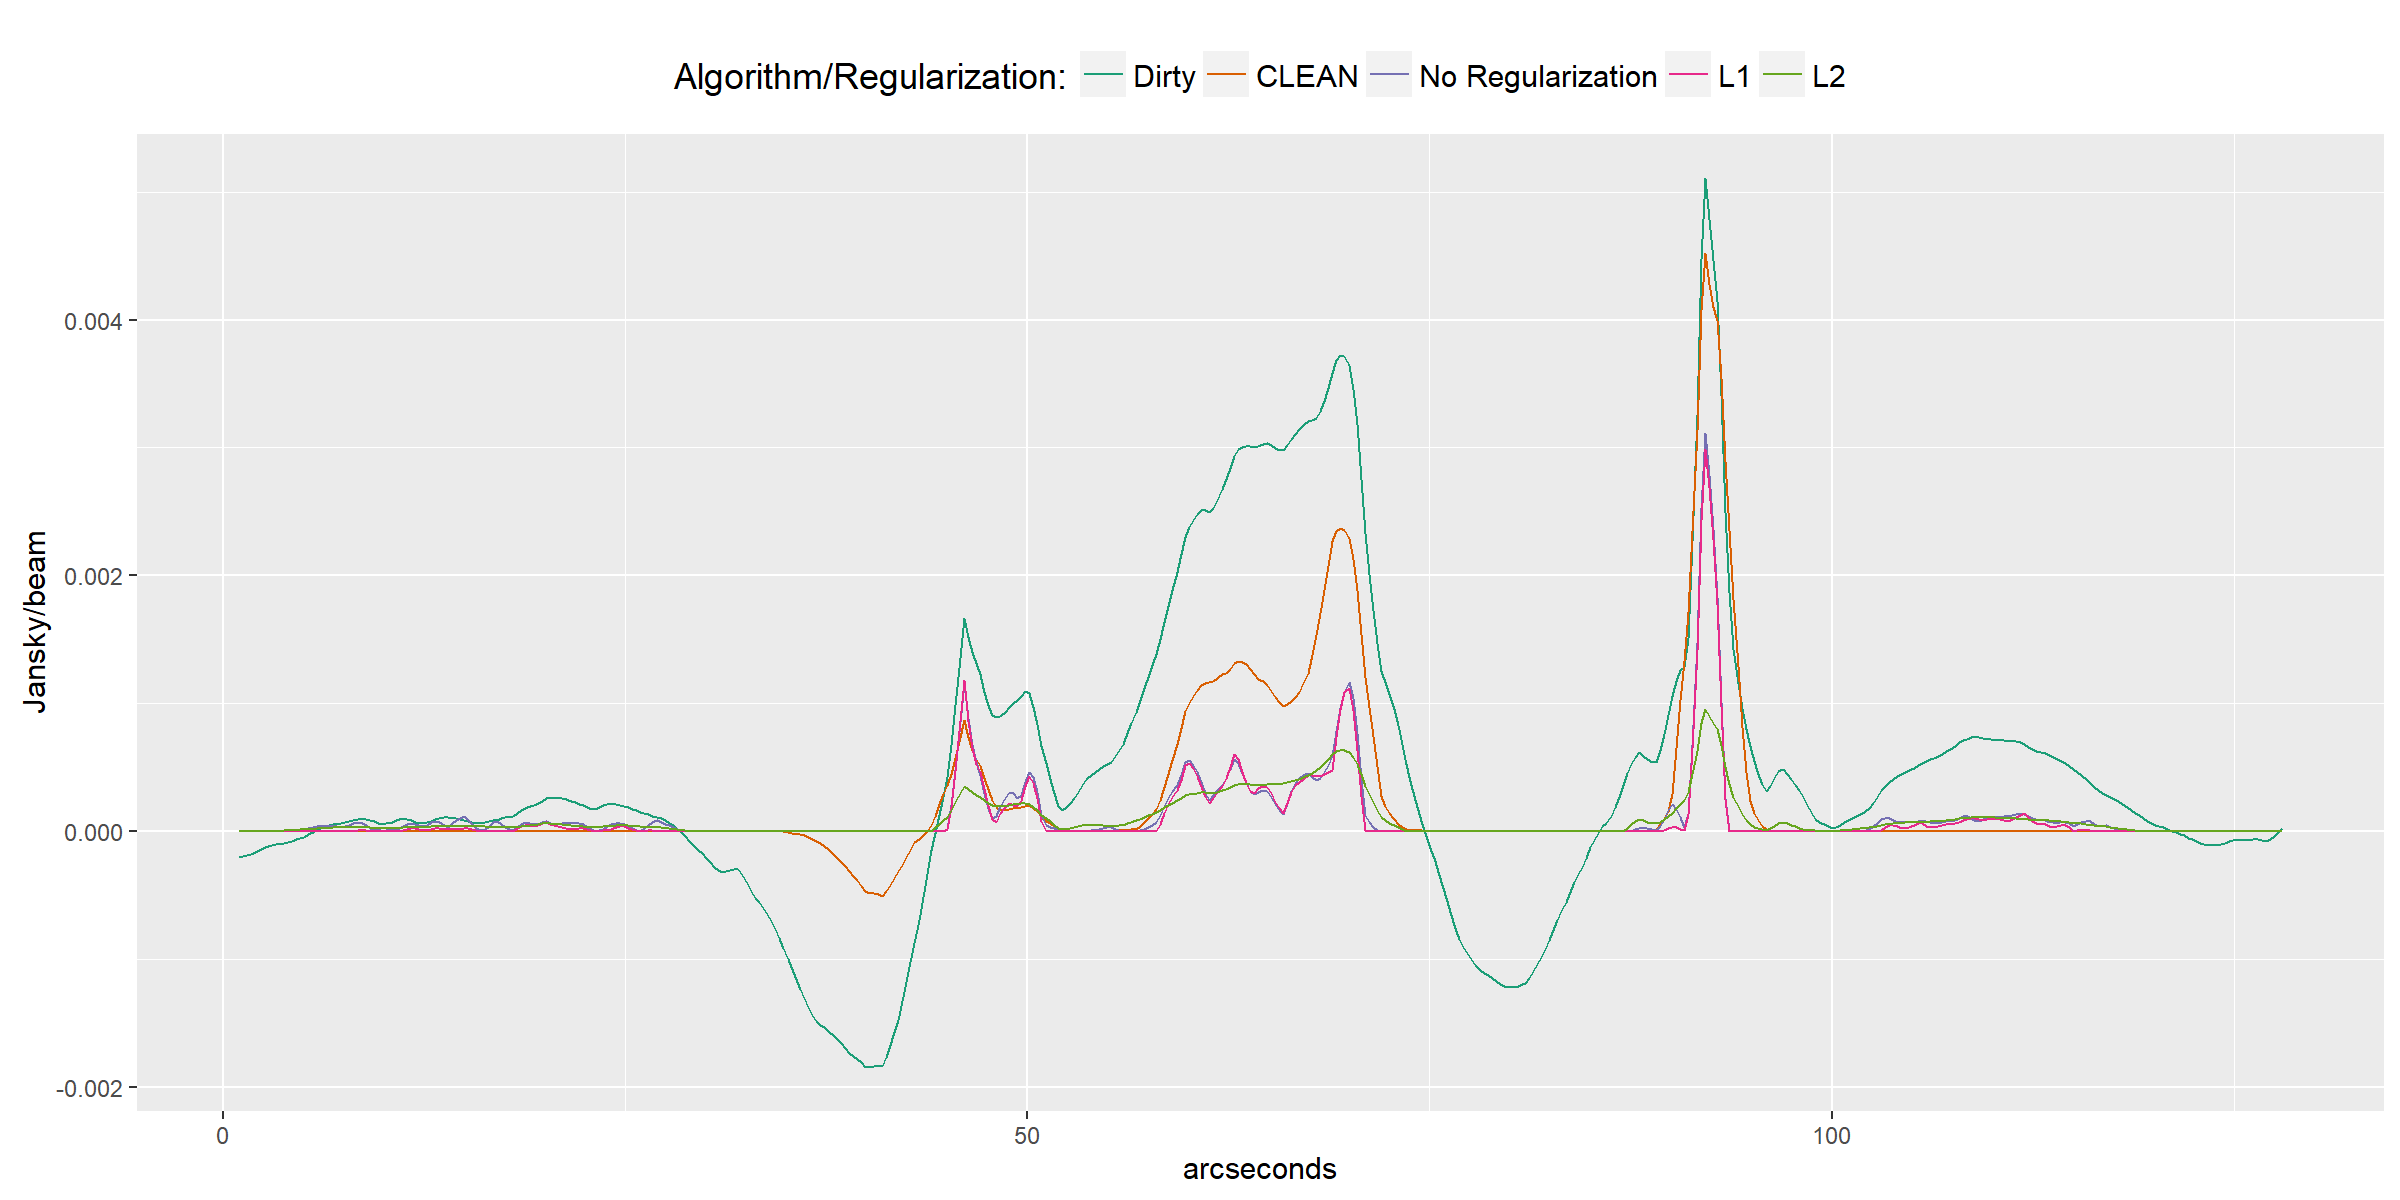
\includegraphics[width=\linewidth, clip]{./chapters/05.results/df1.png}
	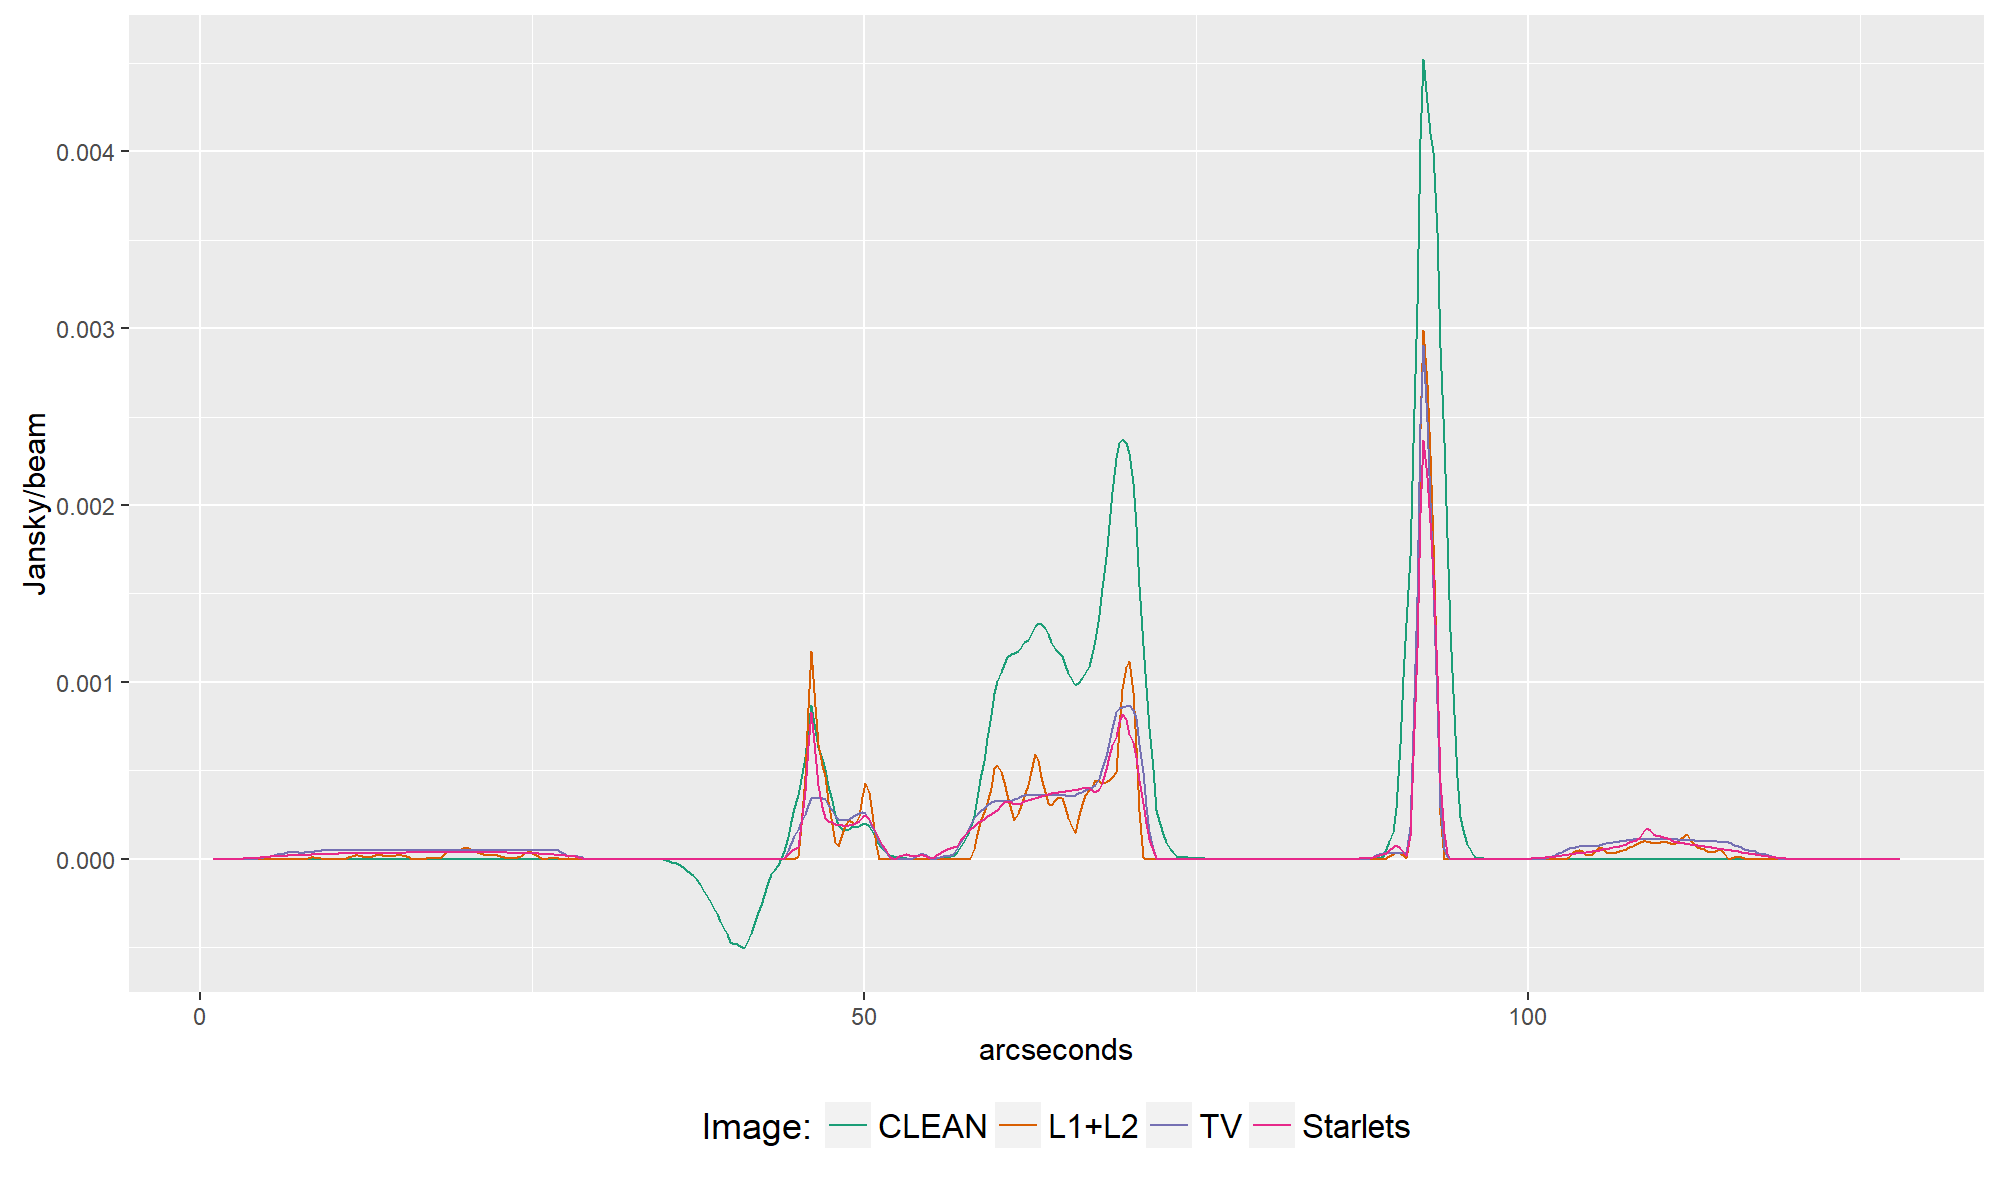
\includegraphics[width=\linewidth, clip]{./chapters/05.results/df2.png}
	\caption{Intensity profile of CLEAN and the different Compressed Sensing Regularizations.}
	\label{res:g55:profile}
\end{figure}

\textbf{CLEAN:} CLEAN detects the brightest point sources, but finds only part of the extended emission. The top half of the "egg" emission is missing. The structures of the remnant are blurred compared to the Compressed Sensing reconstructions. With the parameters of the imaging tutorial, CLEAN models the trench as a region with negative emissions. This is not physically plausible, although the behaviour can be changed with additional parameters. The profile \ref{res:g55:profile} shows that CLEAN accurately reconstructs the flux of the large peaks, although the peaks are wide in comparison.

\textbf{No Regularization:} Detects the egg-head of the remnant and the non-negativity constraint keeps it from modelling the negative trench. It detects the smaller point sources around the remnant, but also detects "fake" extended emissions all around. The profile \ref{res:g55:profile}  shows two smaller peaks in the center (30 arc-minutes) which also appear in the NRAO reconstruction \ref{results:g55:nrao:rec} as do the two small point sources at the edge of the remnant (20 arc-minutes). However, the dirty image has a rise in flux at the borders of the image, which is likely an artefact of the measurement, considering it does not exist in the NRAO reconstruction \ref{results:g55:nrao:rec}.

\textbf{L1:} There is almost no visible difference between no regularization and L1. This is possibly an interaction with the Miller $\lambda$ estimation, since the result of no regularization was used to estimate the $\lambda$ of L1. The L1 regularization removes part of the "fake" extended emission, particularly in the top region, but also a few structures in the center. The peaks in the profile \ref{res:g55:profile} of L1 and no regularization are narrower than CLEAN, although they do not reach the same peak flux. L1 is prone to produce unlikely extended emissions: L1 also tries to approximate extended emissions with a number of faint point sources. This can introduce artefacts like pixel wide holes in extended emissions and produces a "bumpy" profile at the fake extended emissions (at 10 and 50 arc-minutes).

\textbf{L2:} Forces the extended emissions to be more smooth. It also considerably lowers the flux of bright point sources. The profile \ref{res:g55:profile} shows L2 forces the bright peak to widen and lower. The peak is almost as wide as the CLEAN reconstruction. In the remnant center, it blurs structures.

\textbf{L1+L2}: Since L1 does a good job with point sources, but needs to be more continuous for extended emissions, why does one not combine both regularizations? The flexibility of Compressed Sensing Reconstructions allows for it. Sadly, the result is indistinguishable from the L1 regularization. In the dirty image, all pixels are very close to zero (Maximum: 0.0076 in Dirty Image). If the L1 and L2 regularization receive the same $\lambda$, the L1 term dominates. If the dirty image would contain pixels much larger than 1, then the L2 term would dominate.

\textbf{Total Variation:} A simple prior that has its origins in image de-noising. The objective is to reduce the gradients over the image. With an infinite $\lambda$, the Total Variation forces all pixels of the reconstruction to have the same value. The idea of the prior is to work well for both extended emissions and point sources. It has trouble with point sources inside extended emissions. In the profile, it is clearly visible how Total Variations cuts the peaks inside the remnant.

\textbf{Starlets:} Is a more sophisticated prior which also tries to model both point sources and extended emissions. It locates the point sources accurately. In the profile \ref{res:g55:profile} it also finds the faint point sources in the extended emission. However, it also smoothed out the structure inside the remnant. For the LOFAR instrument, the starlet regularization was able to find smaller structures than the antenna beam-width\cite{girard2015sparse}. The smallest starlet has a $5*5$ pixels dimension. For this reconstruction, the antenna beam-width is about two pixels wide. The resolution might be too coarse for the starlet regularization.

CLEAN produces the accurate flux for strong point sources, even though in other reports Total Variation and Starlets reconstructed comparable peak flux to CLEAN \cite{garsden2015lofar}\cite{mcewen2011compressed}.This is due to the implementation in CASA: The PSF CASA produces does not sum up to one. Convolving an image with the PSF increases the total flux, and naturally a deconvolution decreases the flux. CLEAN is the only algorithm that comes close to the measured flux, because in the last iteration, the reconstructed image gets convolved with the beam pattern (usually a 2d gaussian function), which is also not normalized. If we also convolve the Compressed Sensing reconstructions with the beam pattern (and smear away details), the fluxes become similar.

In this example, the L1 normalization was able to find smaller, plausible structures than CLEAN inside the remnant. Outside the remnant, all Compressed Sensing Reconstructions found "fake" extended emissions. The L2 and starlet were also expected to find smaller structures. One possible explanation is that the antenna beam-width is about two pixels wide. Any structure smaller than the beam-width is one pixel wide. For higher resolutions it is expected that L1 introduces more artefacts. The current implementation cannot increase the resolution since it needs a quadratic amount of memory per pixel.


\newpage
\section{Future Compressed Sensing Reconstruction}
Compressed Sensing Reconstructions allow the exchange of priors. New prior knowledge can be incorporated without changing the underlying objective or the optimization algorithm.

Flexibility allows multiple ways to solve the same problem. Optimal solution does not exist yet. 

A proof of Compressed Sensing Reconstruction was implemented in CASA as a deconvolver. It was shown that with Compressed Sensing, one is potentially able to super-resolve sources. However, the current implementation has a quadratic memory requirement, it does not scale to image sizes which are used in practice. New interferometers like MeerKAT will require an even higher amount of pixels. The data amount will scale up by several factors compared to VLA and require scalable image reconstruction. Futhermore, they are built with wide field of view imaging in mind. 

Calibration for these instruments get more complicated. Compressed Sensing Reconstructions are flexible enough and can potentially improve self-calibration tasks.

The next step is to add the effects of wide field of view imaging and see how they scale.



\newpage
\bibliography{mybib}{}
%\bibliographystyle{plain}
\bibliographystyle{unsrt}
\newpage
\listoffigures
\listoftables

\newpage
\input{./chapters/99.attachment/attachment.tex}
\newpage
\section{Ehrlichkeitserklärung}
Hiermit erkläre ich, dass ich die vorliegende schriftliche Arbeit
selbstständig und nur unter Zuhilfenahme der in den Verzeichnissen oder
in den Anmerkungen genannten Quellen angefertigt habe. Ich versichere
zudem, diese Arbeit nicht bereits anderweitig als Leistungsnachweis
verwendet zu haben. Eine Überprüfung der Arbeit auf Plagiate unter
Einsatz entsprechender Software darf vorgenommen werden.\\
Windisch, \today\\[4\baselineskip]
Jonas Schwammberger 

\end{document}